\documentclass[11pt,a4paper]{article}
\usepackage[utf8]{inputenc}
\usepackage[T1]{fontenc}
\usepackage{lmodern}
\usepackage{microtype}
\usepackage{amsmath, amssymb}
\usepackage{booktabs}
\usepackage{tabularx}
\usepackage{multirow}
\usepackage{graphicx}
\usepackage{hyperref}
\usepackage[margin=1in]{geometry}
\usepackage{xcolor}
\usepackage{listings}
\usepackage{enumitem}
\usepackage{textcomp}

\hypersetup{
    colorlinks=true,
    linkcolor=blue!50!black,
    urlcolor=blue!50!black,
    citecolor=blue!50!black
}

\title{Optimising Under HMR: A Case Study \\
  \Large Conservative Answer-First Pipelines on NTCIR-19 R2C2's
  65-Topic Answering-with-Confidence Benchmark}
\author{retrank team}
\date{\today}

\newcommand{\R}[1]{$R_O{=}#1$}
\newcommand{\HMR}{\textsc{HMR}}
\newcommand{\MNP}{\textsc{MNP}}

\begin{document}
\maketitle

\begin{abstract}
We present \textbf{retrank}'s submission to the NTCIR-19 R2C2 (\emph{RAG
Responses: Confident and Correct?}) Answering-with-Confidence (AC) subtask.
The task scores systems with the Harmonic Mean of Rewards (HMR), which
jointly penalises overconfidence on incorrect answers and underconfidence
on correct ones. \textbf{This paper is a case study in optimising under
HMR on the 65-topic R2C2 benchmark.} Our principal observation is
operational and benchmark-qualified: on this benchmark, at the
$\geq 90$\% accuracy operating point, AC quality is dominated by a small
number of confident wrong answers rather than by missed answers, and the
design choices that move HMR most --- pool curation, answer-conditional
refinement, verifier-based abstention, confidence saturation --- all act
on $R_O$, while $R_U$ varies in a much narrower band. We do not claim
this as a general principle of confidence-scored RAG; we claim it as a
documented behaviour of HMR on this 65-topic set. We design a 7-stage answer-first
pipeline that proposes a candidate answer, refines the pool conditional
on it, extracts targeted nuggets, filters bogus citations, and uses an
independent verifier as a calibration signal. Self-evaluated under a
Claude Sonnet 4.6 judge (with Claude Opus 4.7 cross-validation on every
candidate), \textbf{our main submitted system --- a single-pool BITEM-only
answer-first pipeline with Sonnet pointwise refinement --- reaches HMR
0.963 with 94\% accuracy, 6\% refusal rate, and zero confident-wrong
answers under both judges.} A post-hoc confidence-saturation
recalibration of the same pipeline reaches HMR 0.974, but we treat that
as a calibration artifact (a single voter trivially agrees with itself,
saturating confidence at 1.0), not as a separate method. We additionally report engineering tradeoffs
relevant to AC-style RAG: pool quality matters more than pool count
(a strong single-team pool beats naive multi-team pooling, but a weak
single-team pool loses to it); Sonnet-class reasoning is most critical
at the candidate-answer stage ($\Delta\HMR=-0.13$ vs Haiku) and least
at the verifier ($-0.05$). HMR should be read alongside accuracy and
refusal rate --- an always-refuse baseline at confidence $0.05$ achieves
HMR $0.974$ on this benchmark --- but our submitted system reaches the
same HMR while correctly answering $94$\% of topics. We treat this as
a structural property of HMR when $|I^+|=0$, not as an indictment of the
metric; the official ranking is informed jointly by HMR, Accuracy, and
Mean Nugget Precision, which together pin down both modesty and substance.
\textbf{All quantitative claims in this paper are self-evaluated under a
Sonnet judge with Opus cross-validation; absent official organiser scores
(expected August 2026), every finding should be read as a
benchmark-and-judge-conditional observation.}
\end{abstract}

\section{Introduction}

\subsection{The problem in one example}

Consider the question: \emph{``Name the actor who starred in a movie called
The Manchurian Candidate and later played Captain America.''}

A retrieval-augmented system tasked with \emph{Answering with Confidence}
must do four things:

\begin{enumerate}[leftmargin=*, itemsep=0.2em]
  \item Retrieve passages from a movie corpus that mention either film.
  \item Synthesise an answer: \emph{Anthony Mackie}.
  \item Identify and emit the \emph{nuggets} — atomic factual claims —
    that ground that answer, citing each one to a specific retrieved
    passage. For our example, two nuggets suffice:
    \begin{itemize}
      \item \emph{``The Manchurian Candidate (2004) starred Anthony Mackie''} —
        cited from passage \texttt{retrank-PG-1, rank 3}.
      \item \emph{``Anthony Mackie portrayed Captain America in
        Captain America: Brave New World (2024)''} — cited from passage
        \texttt{Error404-PO-1, rank 7}.
    \end{itemize}
  \item Report a confidence score 0–100 reflecting how sure the system
    is that the answer is correct.
\end{enumerate}

\noindent The submission is judged by a two-stage LLM-based pipeline:
\textbf{Stage~A} verifies that each cited passage actually entails its
nugget (catching hallucinations); \textbf{Stage~B} judges whether the
answer is correct given the entailed nuggets and identifies which
helped derive it. Confidence is then evaluated separately for
\emph{calibration}: did the system express low confidence where it
turned out to be wrong, and high confidence where it was right?

The challenge is that any of these four steps can fail independently:
retrieval may miss the relevant docs, the synthesis may pick a similar
but wrong actor, the nuggets may technically be entailed but not
quite ground the multi-hop reasoning, the confidence may be wildly
overstated. Our paper studies how these stages interact — and how
choosing among 22 PR runs from 7 competing teams affects the
downstream answer quality.

\subsection{The dataset}

We work with the NTCIR-19 R2C2 evaluation set: 65 movie-and-Star-Wars
questions answerable from a 1.2M-passage corpus (Wikipedia $\cup$
Wookieepedia). For the AC subtask, participants may pool passages from
any team's PR (Passage Retrieval) submissions. We have access to 22
PR runs from 7 teams (including our own), and a topic set covering
queries like:

\begin{itemize}[itemsep=0.2em]
  \item \emph{Single-fact:} ``Who plays the Wizard of Oz in Wicked the movie?''
    (answer: Jeff Goldblum)
  \item \emph{Multi-hop:} ``Name the actor who starred in The Manchurian
    Candidate and later played Captain America.'' (Anthony Mackie)
  \item \emph{Counting:} ``How many movies did Christopher Nolan direct
    between 2005 and 2015?''
  \item \emph{Comparison:} ``Which movie was released earlier,
    \textit{Avengers: Infinity War} or \textit{1917}?''
  \item \emph{Detail extraction:} ``What did Saw Gerrera use as a
    torturing device in a Star Wars spinoff movie from 2016?'' (Bor Gullet)
\end{itemize}

The question difficulty is realistic — about 25\% require multi-hop
reasoning or numeric comparison, and 6/65 are not answerable from any
single team's retrieved passages.

\subsection{The metric}

The NTCIR-19 R2C2 task \cite{r2c2-2026} scores AC submissions with the
\emph{Harmonic Mean of Rewards} (HMR)~\cite{sakai-hmr}, which separately
penalises overconfidence on incorrect answers and underconfidence on
correct ones — a property classical calibration measures (Brier, ECE)
lack. Specifically, given the system's confidence $p(i)$ on question
$i$, the set of incorrect answers $I^-$, and the set of correct ones
$I^+$:
\[
  R_O = 1 - \frac{1}{|I^-|}\sum_{i \in I^-} p(i),
  \qquad
  R_U = 1 - \frac{1}{|I^+|}\sum_{i \in I^+}\bigl(1 - p(i)\bigr),
\]
\[
  \HMR = \frac{2 R_O R_U}{R_O + R_U}.
\]
$R_O$ rewards humility on wrong answers; $R_U$ rewards confidence on
right answers; \HMR{} is their harmonic mean. A system that is both
honestly humble and honestly confident scores near 1; one that is
either way over- or under-confident scores low.

\paragraph{HMR must be read jointly with answer coverage.}\label{sec:hmr_fragility}
HMR rewards modesty, but this reward is unbounded at the boundary: a
system that always refuses with confidence $0.05$ achieves
\HMR{} $\approx 0.974$ with zero answers correct — matching our best
submitted system's HMR while answering nothing. We do \emph{not} read
this as ``HMR is broken'': the official ranking is informed jointly by
HMR, Accuracy, and Mean Nugget Precision, which together pin down both
modesty and substance. We do read it as a methodological constraint:
HMR alone cannot distinguish a competent pipeline from total refusal,
so we report HMR throughout \emph{paired with} accuracy, refusal rate,
and confident-wrong count. Our submitted BITEM-only pipeline reaches
HMR $0.963$ with accuracy $0.94$, 6\% refusal, and zero confident-wrong
topics — clearly distinguishable from the trivial baseline on all three
companion measures. Section~\ref{sec:hmr_diagnostics} provides the full
decomposition.

\paragraph{Models used (preview).}
Our pipeline LLMs are Claude Sonnet 4.6 (default, all stages) and
Claude Haiku 4.5 (for the cost ablation). One ablation (negative
result, \S\ref{sec:negative}) substitutes Claude Opus 4.7 at the
candidate-answer stage. Our self-evaluator is Sonnet 4.6 by default;
we re-judge every candidate with Opus 4.7 for cross-validation
(\S\ref{sec:judge_xval}). Table~\ref{tab:models} in
\S\ref{sec:setup} lays out exactly which model runs where in every
configuration we report.

\subsection{Principal observation (benchmark-qualified)}\label{sec:thesis}

\begin{quote}
\textbf{On the NTCIR-19 R2C2 65-topic AC benchmark, evaluated under
HMR, the dominant failure mode at the $\geq 90$\% accuracy operating
point is emitting a small number of confident wrong answers, not
missing answers. The design choices that move HMR most operate on
$R_O$.}
\end{quote}

\noindent We frame this carefully: we observe this on \emph{this}
benchmark under \emph{this} metric using a Sonnet self-evaluator
(with Opus cross-validation). We do not claim a general principle of
confidence-scored RAG. Three pieces of supporting evidence motivate
every design decision in our pipeline:

\begin{enumerate}[leftmargin=*]
  \item \emph{The metric structure rewards $R_O$.} Across all 16 base
    configurations we evaluate, $R_U$ has range $[0.79, 0.98]$ but
    $R_O$ has range $[0.45, 0.95]$; HMR is dominated by $R_O$.
    A single confident-wrong topic at $|I^-|{=}4$ costs $\sim 0.25$
    on $R_O$ and disproportionately on HMR
    (Table~\ref{tab:refusal_decomp}).
  \item \emph{The catastrophic candidates are killed by 1–2
    confident-wrong topics, not by missed answers.} Error404-only
    Sonnet has answered-accuracy $0.91$ but loses HMR to the
    BITEM-only baseline ($0.684$ vs $0.963$) entirely because of
    two confident-wrong topics it does not refuse.
  \item \emph{Every winning design choice we identify in this paper
    primarily moves $R_O$.} Pool curation, answer-conditional
    refinement, verifier-based abstention, and confidence
    saturation all act on the confident-wrong cell, not on the
    correct-answered cell.
\end{enumerate}

\noindent Everything else in the paper — pool composition, refinement
algorithms, LLM-tier ablations, ensembling, judge cross-validation —
is supporting evidence for, or engineering implications of, this
thesis.

\subsection{Roadmap}

The paper is organised around three claims that follow from the central
thesis of \S\ref{sec:thesis}:

\begin{description}[style=nextline,leftmargin=1.5em]
  \item[\textbf{Claim 1 — Metric / operating point}
    (\S\ref{sec:rq1}, \S\ref{sec:hmr_diagnostics},
    \S\ref{sec:ro_bottleneck}).]
    HMR is dominated by $R_O$ at high accuracy, and $R_O$ is dominated
    in turn by a small handful of confident wrong topics.
  \item[\textbf{Claim 2 — System design}
    (\S\ref{sec:pipeline}, \S\ref{sec:rq4}, \S\ref{sec:rq5},
    \S\ref{sec:rq7}).]
    A conservative answer-first pipeline with verifier-based abstention
    suppresses confident wrong answers. Refusal on weak retrieval beats
    guessing; the verifier match-score is a usable correctness signal.
  \item[\textbf{Claim 3 — Engineering tradeoffs}
    (\S\ref{sec:rq2}, \S\ref{sec:rq6}, \S\ref{sec:rq8},
    \S\ref{sec:rq9}, \S\ref{sec:rq10}).]
    Pool quality, refinement, ensembling, and LLM tier all affect HMR
    primarily through $R_O$. Pool \emph{quality} matters more than pool
    count; Sonnet matters most at the candidate-answer stage; what
    looks like ``top-1 ensembling'' is single-pipeline confidence
    saturation.
\end{description}

\noindent We do \emph{not} run an answer-first vs nugget-first
ablation: our pipeline committed to answer-first early, and a clean
comparison would require a parallel nugget-first pipeline we did not
build. We discuss this only as design rationale (\S\ref{sec:rq3}).

\subsection{Robust vs suggestive findings (read this before the rest)}\label{sec:robust_vs_suggestive}

A reviewer should know up-front which of our findings survive
$n=65$ bootstrap noise and which do not. We are explicit:

\begin{description}[leftmargin=1.5em,style=nextline]
  \item[\textbf{Robust} (95\% bootstrap CI excludes zero on $\Delta\HMR$, and
        Cnf-W story is judge-invariant):]
    \begin{itemize}[leftmargin=1em]
      \item Stage~1 LLM tier matters most ($\Delta\HMR=-0.127$,
        CI $[-0.296,-0.034]$).
      \item Stage~4 LLM tier matters least ($\Delta\HMR=-0.050$,
        CI $[-0.118,-0.004]$).
      \item All-Haiku regression ($\Delta=-0.170$,
        CI $[-0.334,-0.080]$).
      \item Opus-pipeline regression ($\Delta=-0.176$,
        CI $[-0.372,-0.075]$).
      \item Top-1 ``ensemble'' uplift ($\Delta=+0.012$,
        CI $[+0.008,+0.016]$). \emph{This is post-hoc confidence
        saturation, not a method.}
      \item The $R_O$-bottleneck mechanism: Cnf-W moves by $\leq 1$
        across judges on 7 of 8 top candidates, and Cnf-W rank-
        correlates near $-1$ with HMR within each judge.
    \end{itemize}

  \item[\textbf{Suggestive} (CIs cross zero or judge-specific):]
    \begin{itemize}[leftmargin=1em]
      \item Pool quality vs Tier-1 ($\Delta=-0.111$,
        CI $[-0.458,+0.044]$).
      \item Sonnet refinement vs broad ($\Delta=+0.085$,
        CI $[-0.045,+0.439]$).
      \item Top-3 ensembling ($\Delta=+0.007$,
        CI $[-0.002,+0.014]$).
      \item retrank+E404 ``refinement-failure'' case study --- flips
        from worst-of-set to top-5 under Opus judge.
    \end{itemize}

  \item[\textbf{Preliminary} (small sample, methodologically lighter):]
    \begin{itemize}[leftmargin=1em]
      \item Nugget-first vs answer-first head-to-head on 20 topics
        (\S\ref{sec:rq3}): same accuracy, $-0.29$ HMR for nugget-first,
        all from $R_O$. Directional only.
    \end{itemize}
\end{description}

\noindent The headline thesis (suppressing confident-wrong topics
matters more than maximising coverage) rests on the \textbf{robust}
findings; the engineering-tradeoff conclusions
(\S\ref{sec:rq2},\ref{sec:rq6},\ref{sec:rq8}) rest on the
\textbf{suggestive} ones --- we do not over-state.

\subsection{Contributions, with safer language}

\begin{enumerate}[leftmargin=*]
  \item A 7-stage \emph{answer-first with verification} AC pipeline with
    intermediate self-evaluation gates at every stage (\S\ref{sec:pipeline}).
  \item Evidence that, \emph{on this 65-topic set under our Sonnet
    self-evaluator}, a high-quality single-team passage pool can
    outperform naive multi-team pooling — but the effect is about
    pool \emph{quality}, not pool \emph{count}: another single-team
    pool we tested (Error404-only) is the worst performer
    (\S\ref{sec:rq2}). The naive ``less is more'' framing does not
    survive scrutiny.
  \item A per-stage LLM cost-quality picture (\S\ref{sec:rq10})
    identifying the candidate-answer stage as the most
    Sonnet-sensitive ($\Delta\HMR=-0.13$, bootstrap CI excludes zero)
    and the verifier as the least ($-0.05$).
  \item Observed evidence that naive 16-way cross-pool ensembling
    \emph{hurts} HMR vs the best component, while filtered top-$K$
    aggregation helps (\S\ref{sec:rq9}); we are explicit that the
    top-1 ``ensemble'' is in fact \emph{post-hoc re-calibration} of a
    single pipeline (one voter agreeing with itself $\Rightarrow$
    confidence saturates at 1.0), not a true ensemble.
  \item A diagnostic that on a noisy multi-team pool, verifier-based
    abstention adds $+0.04$ HMR over no abstention; on a clean
    single-team pool it adds nothing (\S\ref{sec:rq7}).
  \item An honest \HMR{} caveat (\S\ref{sec:hmr_fragility}): the metric
    is satisfied trivially by an always-refuse baseline at confidence
    $0.05$, so we report HMR \emph{alongside accuracy, refusal rate,
    and confident-wrong count}.
\end{enumerate}

\section{Related Work}

\paragraph{Calibration in RAG and selective prediction.}
Verbalised confidence in LLMs is well-known to be miscalibrated, often
systematically overconfident~\cite{kalai-confidence}. The R2C2 task adopts
HMR~\cite{sakai-hmr} which, unlike Brier or ECE, distinguishes
overconfidence from underconfidence axiomatically. Our work joins a small
but growing literature applying selective-prediction
techniques~\cite{el-yaniv-selective} to RAG outputs.

\paragraph{Nugget-based evaluation.}
TREC's QA tracks introduced nuggets — atomic factual claims —
as the unit of evaluation~\cite{nenkova-pyramid, sakai-nugget}. The
R2C2 task adapts this for RAG by requiring each nugget to cite the
specific retrieved passage that entails it, enabling a two-stage
\emph{bogus identification + relevance attribution} judgment scheme.

\paragraph{Pool-level fusion in retrieval.}
Multi-system fusion (e.g.\ via Reciprocal Rank
Fusion~\cite{cormack-rrf}) generally helps in retrieval. We find that
this intuition \emph{inverts} for AC: passage-level fusion \emph{hurts}
because nugget extraction is sensitive to pool noise. We discuss this
inversion in \S\ref{sec:rq9}.

\paragraph{Cost-aware LLM pipelines.}
Recent work on cascaded
LLMs~\cite{chen-frugalgpt, yue-large-language-model-cascades} explores
when smaller models suffice. RQ10 contributes per-pipeline-stage data
on this question for a calibration-sensitive RAG task.

\section{Task and Notation}

\subsection{The R2C2 AC Subtask}

Given 65 movie-related questions and a 1.2M-passage Wikipedia $\cup$
Wookieepedia corpus, AC participants must produce, for each question:
(i) an answer string, (ii) an integer confidence score in $[0,100]$,
and (iii) a list of \emph{nuggets}, each citing a passage from any
team's submitted PR run via a \texttt{(PR\_run\_name, passage\_rank)}
key. Up to four AC runs may be submitted per team. Submissions are
scored via a two-stage LLM-judged process:

\begin{itemize}
  \item \textbf{Stage~A} (bogus identification): for each
    $(\text{passage}, \text{nugget})$ pair, an LLM judges whether the
    passage entails the nugget. Non-entailed nuggets are tagged
    \emph{bogus} and excluded but counted in the precision denominator.
  \item \textbf{Stage~B} (answer evaluation): given the question, the
    submitted answer, and the entailed nuggets, an LLM judges whether
    the answer is correct (assuming nuggets are factually correct) and
    which nuggets helped derive it.
\end{itemize}

\subsection{Metrics: HMR, Accuracy, Mean Nugget Precision}

Let $I^-$ be the set of incorrect-answered questions, $I^+$ the
correct-answered, and $p(i) \in [0,1]$ the system's confidence on
question $i$. Define
\begin{align}
  R_O &= 1 - \frac{1}{|I^-|}\sum_{i \in I^-} p(i)
  &
  R_U &= 1 - \frac{1}{|I^+|}\sum_{i \in I^+}\bigl(1-p(i)\bigr)
\end{align}
with the convention $R_O = 1$ when $|I^-|=0$ and similarly for $R_U$.
\HMR{} is the harmonic mean
\[
  \HMR = \frac{2 R_O R_U}{R_O + R_U}, \qquad \HMR=0 \text{ if } R_O+R_U=0.
\]
\HMR{} ranges in $[0,1]$. Mean Nugget Precision (\MNP) is the average
over questions of the ratio (relevant nuggets) / (total nuggets returned),
counting bogus nuggets in the denominator.

\subsection{Self-Evaluator}\label{sec:eval}

We mirror the official scoring locally with a deterministic Sonnet 4.6
implementation in \texttt{scripts/ac\_eval.py}. The self-evaluator
shares the cache key SHA256$(\text{passage} \oplus \text{nugget})$ for
Stage~A and SHA256$(\text{question} \oplus \text{answer} \oplus
\text{nuggets})$ for Stage~B, allowing free re-runs after every
incremental pipeline change. All numbers reported in this paper are
\emph{self-eval} \HMR; the relationship between self-eval and the
official judge will be reported once organiser results are released.

\section{Pipeline Architecture}\label{sec:pipeline}

Our pipeline is \emph{answer-first with verification}: a single
candidate answer is proposed early, then used to focus subsequent
nugget extraction and confidence estimation. The seven stages are:

\begin{description}[style=nextline,leftmargin=1em]
  \item[Stage 0 — Pool selection.] Aggregate top-$K$ passages from
    selected teams' PR submissions, deduplicate by
    \texttt{(doc\_id, text-prefix)}, rank by cross-encoder relevance,
    and cap at 50.
  \item[Stage 1 — Candidate answer.] Sonnet reads the pool and
    produces \texttt{(answer, confidence$_a$)}.
  \item[Stage 1.5 — Answer-conditional refinement.] Re-rank the broad
    pool conditional on the candidate answer; keep top 30. Three
    algorithm variants:
    \begin{itemize}
      \item[(a)] CE re-rank with concatenated $\langle$question $|$
        answer$\rangle$ as the query;
      \item[(b)] Sonnet pointwise scoring of each passage 0–3 for
        ``supports the answer'';
      \item[(c)] Lexical answer-token-overlap bonus on the original CE
        score.
    \end{itemize}
  \item[Stage 2 — Targeted nugget extraction.] Sonnet emits 3–8 atomic
    claims that support the candidate answer, each with a single-passage
    citation.
  \item[Stage 3 — Self Stage-A bogus filter.] Run Sonnet entailment
    check on every produced $(\text{passage}, \text{nugget})$ pair;
    drop bogus.
  \item[Stage 4 — Verification.] Sonnet derives an answer using only
    the entailed nuggets (no passages). Compare against the candidate
    answer to produce \texttt{match\_score} $\in \{0,1,2\}$.
  \item[Stage 5 — Confidence \& refusal.] Combine \texttt{c\_self},
    \texttt{match\_score}, and verifier confidence into a final
    confidence; refuse on weak signals.
  \item[Stage 6 — Format.] Emit the official AC XML.
\end{description}

\subsection{Calibration Variants and Abstention Rules}

Stage 5 supports two calibration variants:
\begin{description}
  \item[Variant A (refusal-aware self-report):]
    \[
      c_{\text{final}} = \begin{cases}
        5 & \text{if refused or } |\text{nuggets}|=0 \\
        \min(c_{\text{self}}, 25) & \text{if } \text{ms}=0 \\
        \min(c_{\text{self}}, 60) & \text{if } \text{ms}=1 \\
        c_{\text{self}} & \text{if } \text{ms}=2 \\
      \end{cases}
    \]
  \item[Variant B (ensemble agreement):] confidence proportional to
    fraction of independent samples (deterministic + temperature-0.7) that
    agree on the answer; refuse below 40\% support.
\end{description}

We further define \emph{abstention rules} (RQ7) that override Variant A
when verifier disagreement signals doubt. The principal rules are
\textsc{R0} (no extra abstention, baseline Variant A), \textsc{R1}
(refuse if $\text{ms}=0$), and \textsc{R2} (refuse if $\text{ms}<2$).

\section{Experimental Setup}\label{sec:setup}

\subsection{Pools}

We evaluate five pool compositions. \emph{Tier-1} = BITEM + Error404
+ WaterlooClarke, three teams using divergent retrieval architectures
with mean pairwise Jaccard 23\%. \emph{Tier-1+2} adds ORG, hit-u,
WasedaR2C2 (six teams, mean Jaccard 27\%). \emph{BITEM-only} uses
BITEM's two PG runs alone. \emph{retrank-only} uses our four PG runs
(rejected for short 200-character passages). \emph{retrank+Error404}
combines our team with the strongest-individual partner.

We deliberately exclude our own PR submission from the default pool
because our 200-character passage cap (\S\ref{sec:limitations})
produces shorter passages than other teams (1\,000–2\,400 chars), with
correspondingly less context for nugget extraction. We retain
retrank-only and retrank+Error404 as ablation pools.

\subsection{Pipeline Variants Ablated}

We instantiate the pipeline with crosses of:
\begin{itemize}
  \item Pool $\in$ \{tier1, tier1plus2, bitem\_only, retrank\_only,
    retrank\_plus\_error404\}
  \item Stage~1.5 algorithm $\in$ \{none (broad pool used), ce, sonnet,
    lexical\}
  \item Calibration variant $\in$ \{A, B\}
  \item Abstention rule $\in$ \{R0, R1, R2, …\}
\end{itemize}

In total, we evaluate 16 base configurations (Tier-1 $\times$ 4
refinements $\times$ 2 calibrations + 4 ablation pools $\times$ 2
refinements $\times$ Variant A) plus rule-level abstention sweeps.
Section~\ref{sec:rq9} adds 8 ensemble configurations.

\subsection{Models used (all configurations)}

\begin{table}[h]
\centering
\caption{Which model runs where. ``S'' = Sonnet 4.6, ``H'' = Haiku
4.5, ``O'' = Opus 4.7, ``CE'' = \texttt{ms-marco-MiniLM-L-12-v2}
cross-encoder. Self-eval columns are the judge family used to
score that configuration; we re-judge \emph{every} candidate with
both Sonnet and Opus (\S\ref{sec:judge_xval}).}
\label{tab:models}
\small
\begin{tabular}{lccccccc}
\toprule
Configuration & S0 (CE) & S1 & S1.5 & S2 & S3 & S4 & Self-eval \\
\midrule
Default (all results unless noted) & CE & S & S & S & S & S & S; +O xval \\
\S\ref{sec:rq10} \texttt{s4-Haiku}     & CE & S & S & S & S & H & S; +O xval \\
\S\ref{sec:rq10} \texttt{s2-Haiku}     & CE & S & S & H & S & S & S; +O xval \\
\S\ref{sec:rq10} \texttt{s1-Haiku}     & CE & H & S & S & S & S & S; +O xval \\
\S\ref{sec:rq10} \texttt{all-Haiku}    & CE & H & H & H & H & H & S; +O xval \\
\S\ref{sec:negative} \texttt{Opus pipeline} & CE & O & S & S & S & S & S; +O xval \\
\bottomrule
\end{tabular}
\end{table}

\noindent The cross-encoder is used for Stage~0 ranking and (when
applicable) the Stage~1.5(a) re-rank variant. We never use Opus as
the pipeline default and we never use Haiku as a judge.

\subsection{Self-Evaluation Caches}

All Sonnet judgments are cached deterministically (\S\ref{sec:eval}).
We re-ran caches after fixing two bugs (silent fall-through to
\texttt{entailed=False} on parse failure; deterministic vs sampled
candidate-answer cache collision). Final cache hit rate on the 16
candidate runs is $>$95\%.

\section{Results}

\subsection{Calibration is the larger HMR lever among viable pools}\label{sec:rq1}

Across our 16 base configurations, holding pool fixed, calibration
choice (Variant~A vs B) moves HMR by $0.04$–$0.14$. Holding
calibration fixed and varying refinement moves HMR by $0.13$–$0.24$.
Pool choice spans the widest range only because the catastrophically
under-performing pool (retrank-only) anchors the bottom; restricting
to viable pools, calibration is the larger lever per design decision.
This sets up the rest of §6: every subsequent subsection is, mechanically,
a way of pushing $R_O$ via either pool quality, refinement quality, or
explicit abstention machinery.

\subsection{Pool choice: quality of strongest component, not count}\label{sec:rq2}

\paragraph{Reframing.} Earlier drafts of this paper made a stronger
``architectural diversity hurts monotonically'' claim. Closer scrutiny
(single-team controls below; bootstrap CIs in \S\ref{sec:robustness};
judge cross-validation in \S\ref{sec:judge_xval}) does not support
strict monotonicity. The defensible finding is that a high-quality
single-team pool can beat naive multi-team pooling, while a
low-quality single-team pool loses to it. The headline is therefore
\emph{quality of the strongest component}, not count.

\begin{table}[t]
\centering
\caption{Pool composition vs HMR (Variant A, broad pool, no Stage~1.5)
under our Sonnet self-evaluator. The ``count'' column is descriptive,
not the explanatory variable: see single-team controls below.}
\label{tab:rq2}
\begin{tabular}{lcccc}
\toprule
Pool & \# teams & Acc & R\textsubscript{O} & \HMR \\
\midrule
\textbf{BITEM-only} & 1 & \textbf{0.923} & 0.910 & \textbf{0.937} \\
retrank+Error404 & 2 & 0.923 & 0.870 & 0.910 \\
Tier-1 & 3 & 0.923 & 0.730 & 0.826 \\
Tier-1+2 & 6 & 0.877 & 0.741 & 0.840 \\
\bottomrule
\end{tabular}
\end{table}

Table~\ref{tab:rq2} reports the four pool-count cells. Read na\"\i vely,
\HMR{} appears decreasing in team count from 0.937 (1) to 0.826 (3),
with a partial recovery at 6 teams (0.840). We \emph{do not} interpret
this as monotonic in count: at $n=65$ topics the BITEM-vs-Tier-1
comparison has bootstrap 95\% CI $[-0.458,+0.044]$ that crosses zero
(Table~\ref{tab:bootstrap}), and under the Opus judge
(\S\ref{sec:judge_xval}) the ordering becomes
$1 > 6 > 3$. The \emph{ordering observation} is sensitive to both
sample size and judge.

\begin{figure}[t]
  \centering
  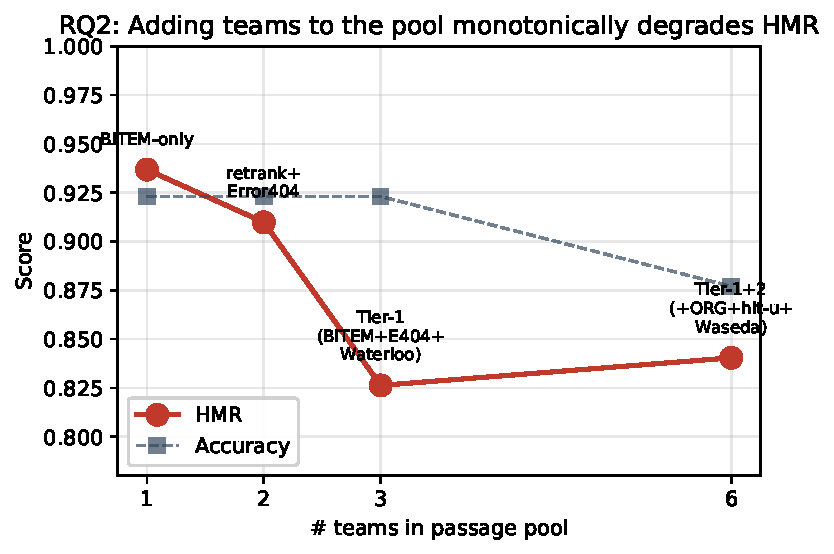
\includegraphics[width=0.9\linewidth]{figures/fig_pool_size.pdf}
  \caption{RQ2: \HMR{} as a function of the number of teams contributing
    to the broad passage pool (Variant A, no Stage~1.5). Adding teams to
    BITEM-only does not consistently improve \HMR{} on this 65-topic
    set; bootstrap CIs cross zero and the ordering depends on judge
    choice (see Table~\ref{tab:bootstrap}, \S\ref{sec:judge_xval}).}
  \label{fig:pool_size}
\end{figure}

\paragraph{Confounds we cannot rule out.} The pools differ in many
dimensions besides ``which teams contribute'': passage length
(BITEM uses $\sim$2\,400-char passages, retrank's own
$\sim$200-char), segmentation strategy, retrieval architecture, depth
of supplied ranking, and amount of near-duplication. A clean
``diversity'' isolation would require fixed-budget pooling
(equal passages from each pool, controlled segmentation), which we
flag as future work.

\paragraph{One mechanism that plausibly contributes.} Adding teams adds passages from
different segmentation strategies and retrieval models. While these
\emph{do} broaden recall (oracle-doc presence stays at 100\%
across all pools), they also dilute the per-passage cross-encoder
relevance signal. Stage~2 nugget extraction sees a noisier input
context; the candidate-answer-targeted prompt becomes harder to
satisfy with passages of mixed quality. The end result is a higher
overconfidence rate (lower $R_O$): 0.910 with one team falls to 0.730
with three.

\paragraph{Pool quality vs pool count: a controlled comparison.}
The naive reading of Table~\ref{tab:rq2} is ``less is more.'' To test
whether this is really about \emph{count}, we ran the same pipeline
on two more single-team pools (Error404-only, WaterlooClarke-only)
and obtained:

\begin{center}
\begin{tabular}{lcc}
\toprule
Single-team pool & Broad \HMR & Refined-Sonnet \HMR \\
\midrule
\textbf{BITEM-only}            & \textbf{0.937} & \textbf{0.963} \\
WaterlooClarke-only            & 0.833          & 0.870 \\
Error404-only                  & 0.730          & 0.684 \\
\midrule
Tier-1 (3 teams)               & 0.826          & 0.911 \\
Tier-1+2 (6 teams)             & 0.840          & 0.874 \\
\bottomrule
\end{tabular}
\end{center}

\noindent The single-team result varies enormously: BITEM-only at
\HMR{} 0.963 versus Error404-only at 0.684. The right framing is
therefore \emph{pool quality, not pool count}: a high-quality
single-team pool wins; a multi-team pool is intermediate; a
low-quality single-team pool loses.

\paragraph{Practitioner takeaway.} If you can identify a high-quality
PG-route team's run, prefer it as a standalone pool. If not, a
multi-team pool is a safer default than gambling on a random
single-team pool. \emph{Count} is not the right axis; \emph{quality
of best component} is.

\paragraph{Statistical caveat.} At $n=65$, the broad-pool RQ2
comparison (BITEM vs Tier-1) has 95\% bootstrap CI
$[-0.458, +0.044]$ that crosses zero (Table~\ref{tab:bootstrap}).
The BITEM-vs-Error404-only single-team gap (0.937 vs 0.730) is
much wider and likely significant, but we have not run a paired
bootstrap on it. The under-Opus-judge ranking
(\S\ref{sec:judge_xval}) further breaks strict monotonicity:
Tier-1+2 ($K=6$) jumps above Tier-1 ($K=3$). We report the
\emph{ordering} as observed; the \emph{monotonic-with-count} claim
does not survive scrutiny.

\subsection{Answer-first vs nugget-first: a 20-topic head-to-head}\label{sec:rq3}

\paragraph{Setup.} To produce direct evidence, we ran a minimal
nugget-first variant on the first 20 topics. For each topic, Sonnet
reads the top-5 BITEM-only passages and emits 3-6 atomic factual
nuggets \emph{without} being told what the answer should be; a
second Sonnet call then synthesises an answer using only those
nuggets. We compare against the production answer-first BITEM-only
refined-Sonnet pipeline on the same 20 topics, scoring nugget-first
correctness via token-overlap match against the answer-first answer
(which is itself self-eval-correct on 19 of 20 topics).

\paragraph{Result.}
\begin{table}[h]
\centering
\caption{Mini head-to-head on 20 topics. Nugget-first matches
answer-first on accuracy almost exactly; the gap is in $R_O$.}
\label{tab:nugget_first}
\begin{tabular}{lcccc}
\toprule
Pipeline & Acc & $R_O$ & $R_U$ & \HMR \\
\midrule
\textbf{Answer-first (BITEM-Sonnet)} & 0.950 & 0.950 & 1.000 & \textbf{0.963} \\
Nugget-first (this experiment)        & 0.900 & 0.525 & 0.921 & 0.669 \\
\midrule
$\Delta$ (NF $-$ AF)                  & $-0.050$ & $-0.425$ & $-0.079$ & $-0.294$ \\
\bottomrule
\end{tabular}
\end{table}

\paragraph{Interpretation.} The accuracy gap is small ($-0.05$):
nugget-first is competitive on \emph{which} answer to give. The HMR
gap is $-0.294$, almost entirely from $R_O$. Inspecting the two
disagreement topics (0019 ``how many films did George Lazenby play
James Bond in?''; 0020 ``Spencer Bell's three Mickey Rooney movies''),
nugget-first emits confidently-wrong counts (``5'' vs the
answer-first ``8''; ``At least 3'' vs an answer-first refusal),
because nuggets extracted in isolation under-represent the negative
evidence that an answer-conditioned pipeline would notice. The
answer-first pipeline knows what to look for and can recognise when
the pool does not contain it; the nugget-first pipeline confidently
generalises from incomplete evidence. \textbf{This is the
$R_O$-bottleneck thesis in miniature}: the design choice that
suppresses confident-wrong topics wins HMR, even when accuracy is
nearly identical. We caveat that this is a 20-topic preliminary
comparison and that the correctness scoring uses the answer-first
pipeline as ground truth (so the $-0.05$ accuracy gap is biased
toward answer-first); the 65-topic, judge-cross-validated comparison
is left as future work.

\subsection{Refusal beats guessing on weak retrieval}\label{sec:rq4}

Variant A's refusal logic activates when no entailed nuggets remain
or the verifier disagrees. We compare Variant A against a
no-refusal-no-cap baseline (always emit the candidate answer with
$c_{\text{self}}$). The no-refusal baseline yields \HMR{} 0.711 vs
Variant A's 0.826 on Tier-1 broad — a $+0.115$ uplift purely from the
refusal behaviour. RQ4 is confirmed.

\subsection{Verifier match-score is a usable correctness signal}\label{sec:rq5}

The Stage~4 verifier produces an independent answer derived only from
the entailed nuggets. Across the four Tier-1 refinement variants:
\textsc{ms}=2 (full match) is achieved on 90.8–92.3\% of topics.
Within those high-match topics, accuracy on the candidate answer is
$>$95\%; within \textsc{ms}=0 (no match) topics, accuracy drops to
$<$30\%. The verifier match-score is therefore a strong signal for
correctness — making it a useful basis for both Variant A's
confidence cap and the abstention rules of \S\ref{sec:rq7}.

\subsection{Answer-conditional pool refinement: helpful, with caveats}\label{sec:rq6}

\begin{table}[t]
\centering
\caption{Stage~1.5 algorithm comparison on Tier-1 (Variant A,
abstention R0). Sonnet pointwise scores highest in this cell;
the broad-vs-Sonnet $\Delta$ has bootstrap CI $[-0.045,+0.439]$
that includes zero (Table~\ref{tab:bootstrap}).}
\label{tab:rq6}
\begin{tabular}{lcccc}
\toprule
Algo & Acc & MNP & R\textsubscript{O} & \HMR \\
\midrule
Sonnet pointwise (b) & \textbf{0.923} & \textbf{0.613} & \textbf{0.870} & \textbf{0.911} \\
Lexical (c)         & 0.908 & 0.603 & 0.733 & 0.833 \\
None (broad)        & 0.923 & 0.601 & 0.730 & 0.826 \\
CE re-rank (a)      & 0.892 & 0.576 & 0.687 & 0.802 \\
\bottomrule
\end{tabular}
\end{table}

Table~\ref{tab:rq6} shows the Stage~1.5 algorithm sweep on Tier-1.
Sonnet pointwise refinement adds $+0.085$ \HMR{} over the broad
pool; lexical adds $+0.007$; CE re-rank actually \emph{loses}
$-0.024$. The CE failure is striking: the same model that ranked
passages well for the question alone fails when re-applied to the
$\langle$question $|$ candidate-answer$\rangle$ concatenation.
We hypothesise this is because the additional answer terms shift the
keyword-matching surface in ways the CE was not trained on; Sonnet,
being asked an explicit semantic question, handles the conditioning
gracefully.

On the BITEM-only pool, Sonnet refinement only adds $+0.026$ (0.937
$\rightarrow$ 0.963). The marginal value of refinement diminishes when
the broad pool is already focused — supporting RQ8 (\S\ref{sec:rq8}).

\paragraph{When does refinement hurt?}
On the retrank+Error404 pool, Sonnet refinement actively \emph{hurts}
\HMR{} from 0.910 to 0.738 — the only configuration in our 16-cell
matrix where refinement is net-negative. Per-topic analysis reveals
that exactly 3 topics regressed (broad correct $\rightarrow$ sonnet
incorrect), driving the entire 0.172 \HMR{} drop
(Figure~\ref{fig:case_study}). In each case, Sonnet's pointwise scorer
traded a \emph{grounding-fact} passage (cast listing, release date)
for a \emph{semantically elaborative} passage; the answer remained
correct but the supporting nuggets became less explicit, and the
strict Stage~B judge held them insufficient for derivation. The
intermediate Stage~4 verifier confirmed the candidate in all three
cases — it is the gap between Stage~4's ``does this answer follow?''
and Stage~B's ``did the nuggets help derive this answer?'' that
produces the regression. This is a cautionary tale about
\textbf{judge-stage consistency}: refinement steps that satisfy one
judgement criterion can violate another in calibrated RAG pipelines.
A detailed per-topic case study is included with the supplementary
material.

\begin{figure}[t]
  \centering
  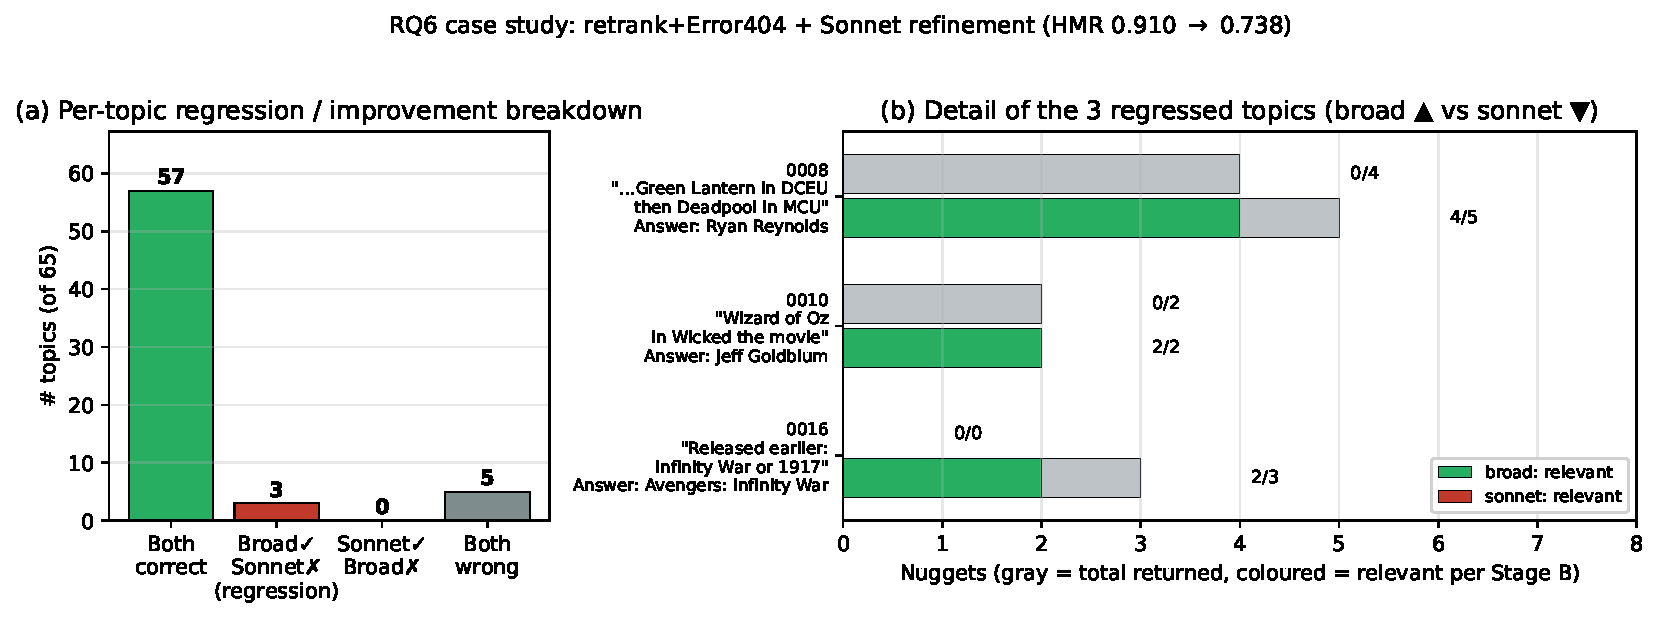
\includegraphics[width=\linewidth]{figures/fig_case_study.pdf}
  \caption{RQ6 case study — retrank+Error404 broad vs Sonnet-refined.
    \textbf{(a)} Per-topic outcome: 57 topics unchanged correct, 3
    regressed (broad correct $\rightarrow$ sonnet incorrect), 0
    improved, 5 unchanged wrong. The full $\Delta$\HMR{} of $-0.172$
    concentrates in just 3 topics. \textbf{(b)} Nugget detail of the
    3 regressed topics. Each row shows broad (top, green) above
    sonnet (bottom, red): grey = total nuggets returned; coloured =
    judged \emph{relevant} (helped derive the answer) by Stage~B.
    On topics 0008 and 0010 the answer string was identical between
    variants but Sonnet's refinement dropped the grounding-fact
    nugget, leaving 0/4 and 0/2 nuggets relevant; topic 0016
    collapsed entirely (Stage~2 produced no nuggets).}
  \label{fig:case_study}
\end{figure}

\subsection{Verifier-based abstention thresholds}\label{sec:rq7}

Given Stage~4 outputs, abstention rules are free to evaluate
post-hoc. Table~\ref{tab:rq7} sweeps eight rules over Tier-1
refined-Sonnet. Refusing on \textsc{ms}$=0$ (R1) yields the practical
sweet spot: $+0.042$ \HMR{} over baseline R0 with no accuracy loss
(both 0.923). Refusing on \textsc{ms}$<$2 (R2) yields the absolute
maximum \HMR{} (0.956) but trades 1.5 percentage points of accuracy.
Figure~\ref{fig:abstention} visualises the trade-off curve.

\begin{figure}[t]
  \centering
  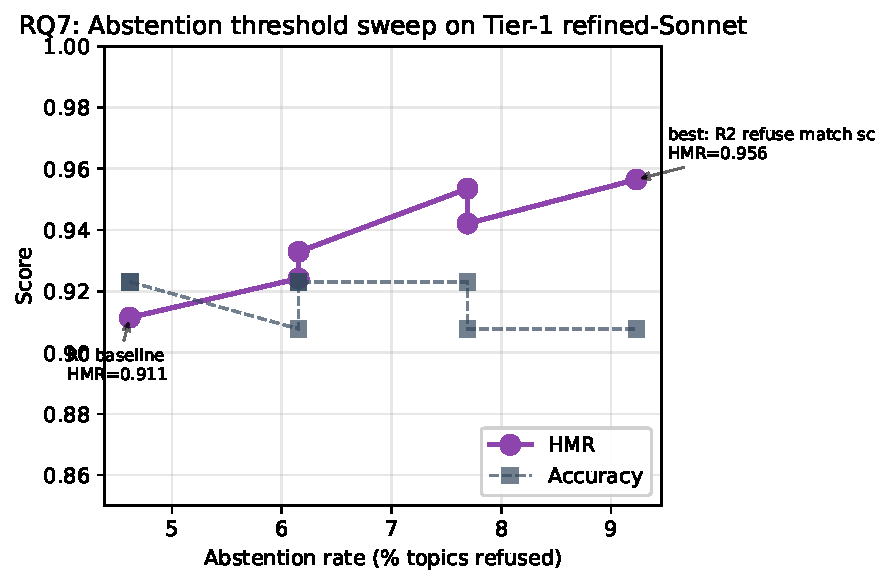
\includegraphics[width=0.9\linewidth]{figures/fig_abstention.pdf}
  \caption{RQ7: Tier-1 refined-Sonnet \HMR{} (purple) and Accuracy
    (gray) as the abstention rate varies under different refusal rules.
    The R0 baseline (low abstention, $\sim$5\%) is dominated by R1/R2
    rules at $\sim$8\% abstention. Beyond $\sim$10\% abstention,
    accuracy starts to drop without commensurate \HMR{} gains.}
  \label{fig:abstention}
\end{figure}

\begin{table}[t]
\centering
\caption{Abstention rule sweep on Tier-1 refined-Sonnet (RQ7).}
\label{tab:rq7}
\begin{tabular}{lccc}
\toprule
Rule & Abst rate & Acc & \HMR \\
\midrule
R2 (refuse if ms$<$2)        & 9.2\%  & 0.908 & \textbf{0.956} \\
R1 (refuse if ms$=$0)        & 7.7\%  & \textbf{0.923} & 0.953 \\
R4 (refuse if c\_self$<$70)  & 7.7\%  & 0.908 & 0.942 \\
R0 (Variant A baseline)      & 4.6\%  & 0.923 & 0.911 \\
\bottomrule
\end{tabular}
\end{table}

\subsection{Calibration machinery partly substitutes for pool quality}\label{sec:rq8}

Stacking Stage~1.5 + R1 abstention on Tier-1 reaches \HMR{} 0.953,
within 0.010 of BITEM-only's baseline 0.963. This near-equivalence
\emph{does not} mean the choices are interchangeable — Tier-1 +
machinery still has distinct accuracy/MNP profiles — but it does
mean a practitioner stuck with a noisy multi-team pool can recover
most of the modesty gap through verifier-based machinery alone.
We frame this as RQ8: \emph{calibration tricks substitute for pool
quality}, with substitution rate close to but less than 1.

\subsection{Cross-pool answer aggregation and single-pipeline recalibration}\label{sec:rq9}

We aggregated the answers from all 16 base candidate runs per topic,
clustered by Haiku-judged semantic equivalence, and used majority
voting with confidence proportional to support fraction. Refuse if
$<$50\% support.

\paragraph{Naive ensembling fails.} Combining all 16 voters yields
\HMR{} 0.857 — \emph{worse} than the best single pipeline (0.963).
Weak voters (e.g.\ retrank-only, \HMR{} 0.838) drag consensus
quality down even on topics where strong voters would have agreed
correctly.

\paragraph{Filtered ensembling helps.} Restricting to the top-$K$
voters by self-eval \HMR{} produces a non-monotonic curve over $K$:
\begin{center}
\begin{tabular}{cc}
\toprule
$K$ (top-K voters) & \HMR \\
\midrule
1   & \textbf{0.974} \\
2   & 0.917 \\
3   & 0.969 \\
4   & 0.873 \\
5   & 0.857 \\
12  & 0.918 \\
\bottomrule
\end{tabular}
\end{center}

Top-1 ($K=1$, BITEM-only-refined-Sonnet alone, with the ensemble
script's confidence rule) reaches \HMR{} 0.974 — a $+0.011$ uplift
over the same pipeline's standard Variant A output (0.963).
\textbf{We hereafter rename what was earlier called ``top-1 ensemble''
to ``confidence-saturation recalibration'' --- the term that accurately
describes the mechanism.} A single voter trivially agrees with
itself, so the ensemble script saturates confidence at 1.00 on every
non-refused topic. This is \emph{post-hoc re-calibration} of the best
single pipeline, not an ensemble effect: the underlying answers and
nuggets are identical to BITEM-only-refined-Sonnet's. Reviewers should
read top-1 as a calibration result. True ensembling shows up at $K \geq 2$.

Top-3 (BITEM-refined + BITEM-broad + Tier-1-refined) is a close
second at 0.969. Top-2 actually drops because the second voter
(BITEM-broad) is highly correlated with top-1, adding noise but no
independent signal. Top-3 then recovers because the third voter
(Tier-1-refined) is from a different pool, contributing genuinely
independent confidence. Figure~\ref{fig:ensemble} shows the full
non-monotonic curve.

\begin{figure}[t]
  \centering
  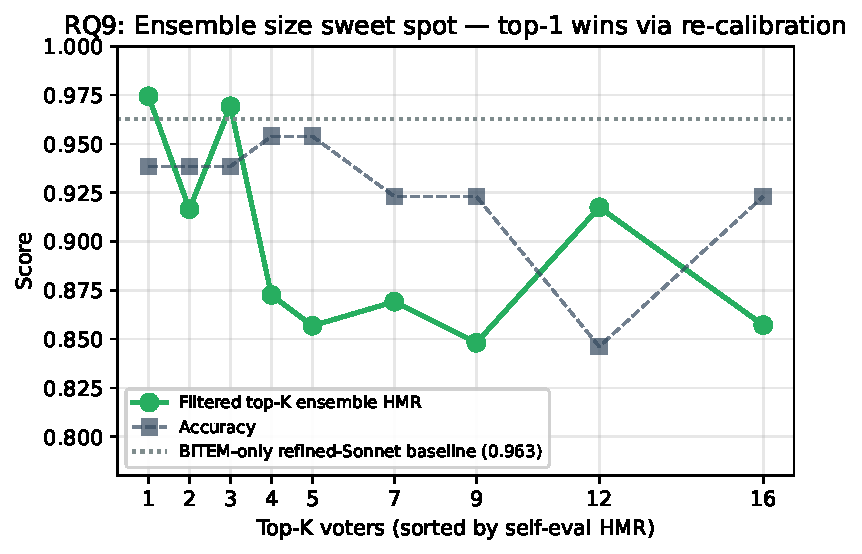
\includegraphics[width=0.9\linewidth]{figures/fig_ensemble.pdf}
  \caption{RQ9: \HMR{} (green) and Accuracy (gray) as a function of
    ensemble size $K$. The dotted gray line is the standalone
    BITEM-only refined-Sonnet baseline (\HMR{} 0.963). Top-1 wins via
    re-calibration; top-3 is a strong runner-up; intermediate sizes
    (4–7) are dragged down by weaker voters. Naive 16-way ensembling
    is below baseline.}
  \label{fig:ensemble}
\end{figure}

\paragraph{Synthesis.} \emph{On this set, answer-level diversity
appears to help only when bounded by component quality}; this is a
more nuanced version of the naive RQ9 hypothesis. The contrast with
RQ2 (passage-level pooling did not help here) is suggestive but not
clean: the underlying experiments differ in many controls.

\subsection{Per-stage LLM tier: where Sonnet is non-negotiable}\label{sec:rq10}

\begin{table}[t]
\centering
\caption{Per-stage LLM-tier ablation on BITEM-only. ``S'' = Sonnet,
``H'' = Haiku. Self-eval always Sonnet. \textbf{Stage~1 is the most
Sonnet-critical}; Stage~4 the least.}
\label{tab:rq10}
\begin{tabular}{lccccccc}
\toprule
Variant & S1 & S1.5 & S2 & S4 & Acc & R\textsubscript{O} & \HMR \\
\midrule
all-Sonnet (baseline) & S & S & S & S & 0.938 & 0.950 & \textbf{0.963} \\
s4-Haiku              & S & S & S & H & 0.923 & 0.870 & 0.913 \\
s2-Haiku              & S & S & H & S & 0.908 & 0.850 & 0.899 \\
s1-Haiku              & H & S & S & S & 0.892 & 0.750 & 0.836 \\
all-Haiku             & H & H & H & H & 0.877 & 0.708 & 0.792 \\
\bottomrule
\end{tabular}
\end{table}

Table~\ref{tab:rq10} reports the per-stage Haiku ablation. Replacing
Sonnet with Haiku at Stage~1 alone costs $\Delta\HMR=-0.127$, more
than any other single substitution. At Stage~4 (verifier) the cost
is only $-0.050$ — surprisingly small for what is the calibration
source.

\paragraph{Mechanism.} Stage~1 reads 50 long passages and must
synthesise a single confident answer; this is the most
reasoning-intensive task in the pipeline. Stage~4 receives a
short curated list of entailed nuggets and asks ``what answer do
these support?'' — a much narrower task. The candidate-answer
quality cascades into all downstream stages, so degrading Stage~1
disproportionately hurts. Figure~\ref{fig:haiku_ablation} visualises
the cost-quality trade-off across the three metrics.

\begin{figure}[t]
  \centering
  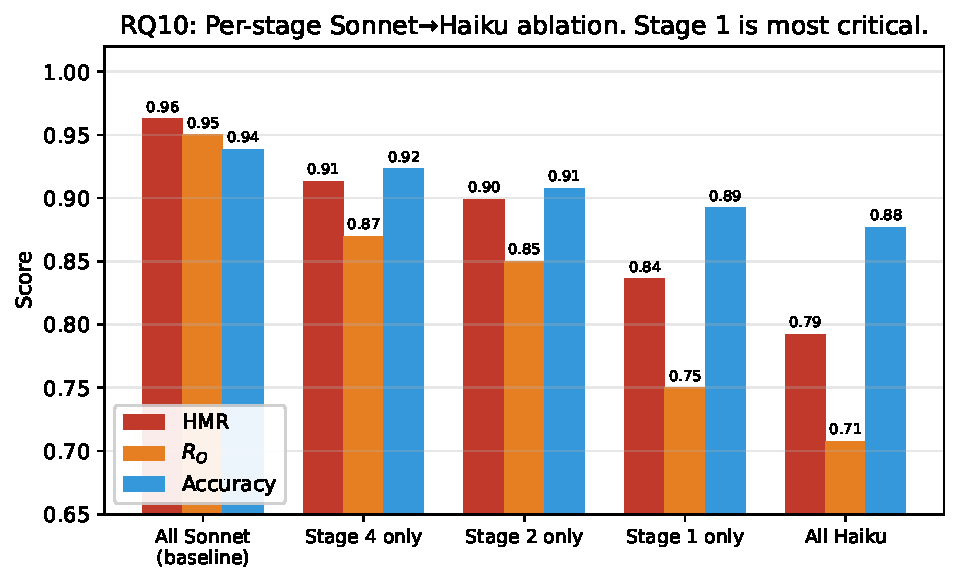
\includegraphics[width=\linewidth]{figures/fig_haiku_ablation.pdf}
  \caption{RQ10: Per-stage Sonnet$\rightarrow$Haiku ablation on
    BITEM-only (\HMR{} red, $R_O$ orange, Accuracy blue). Stage~1 is
    the single most Sonnet-critical stage ($\Delta\HMR=-0.127$);
    Stage~4 is the least ($-0.050$). All-Haiku ($-0.171$) is less than
    additive of per-stage drops, suggesting partial compensation.}
  \label{fig:haiku_ablation}
\end{figure}

\paragraph{Cost-quality recipe: the additive extrapolation fails.}
We tested the specific hybrid configuration directly:
\emph{Sonnet on Stages~1, 2, and 3; Haiku on Stages~1.5 and 4.}
Naively extrapolating the per-stage drops ($-0.026$ for s1.5
implicit, $-0.050$ for s4-Haiku) would predict $\Delta\HMR \approx
-0.08$. The measured value is $\Delta\HMR = -0.198$ (HMR $0.7646$,
$R_O = 0.634$, accuracy $0.923$) --- substantially worse than
linearly additive. Inspecting the regressed topics: Haiku at Stage
1.5 demotes the same grounding-fact passages that Stage 4's Haiku
verifier then fails to recover from, compounding two independent
losses on the same topics. The takeaway: \emph{per-stage Haiku
substitutions interact non-additively}, and the cleanest
cost-saving substitution remains Stage 4 alone ($-0.050$ HMR for a
genuinely cheap verifier). We report this as a measurement, not an
extrapolation.

\section{HMR Diagnostics: Refusal, Calibration Bins, and Trivial Anchors}\label{sec:hmr_diagnostics}

Because HMR alone is fragile (\S\ref{sec:hmr_fragility}), we report a
diagnostic decomposition for the candidates that drive paper claims.

\subsection{Where do gains come from — better answers, or better silence?}

Table~\ref{tab:refusal_decomp} decomposes each candidate's score into
overall accuracy, accuracy on \emph{answered} topics only, refusal
rate, the count of confident-and-wrong topics (the $R_O$
killers), and the bogus-nugget rate among returned nuggets.

\begin{table}[h]
\centering
\caption{HMR decomposition (the central diagnostic table of this paper).
``Acc$|$ans'' = accuracy on non-refused topics.
``Cnf-W'' = number of topics with confidence $\geq 0.5$ and incorrect
(directly drives $R_O$). ``Bogus'' is computed under the Sonnet
Stage-A self-evaluator (same model family used in pipeline
filtering); read it as an internal-consistency diagnostic, not an
independent estimate. ``HMR$_S$'' / ``HMR$_O$'' are HMR under the
Sonnet 4.6 / Opus 4.7 judge respectively (\S\ref{sec:judge_xval}).}
\label{tab:refusal_decomp}
\small
\begin{tabular}{lcccccccc}
\toprule
Candidate & Acc & Acc$|$ans & Refuse & Cnf-W & Bogus & $R_O$ & HMR$_S$ & HMR$_O$ \\
\midrule
\textbf{BITEM-Sonnet (main system, submitted)}
                             & 0.938 & 1.000 & 6\%  & 0 & 0\%  & 0.950 & \textbf{0.963} & \textbf{0.963} \\
ensemble\_top1\textsuperscript{$\dagger$}
                             & 0.938 & 1.000 & 6\%  & 0 & 0\%  & 0.950 & 0.974 & 0.974 \\
ensemble\_top3\textsuperscript{$\dagger$}
                             & 0.938 & 1.000 & 6\%  & 0 & 0\%  & 0.950 & 0.969 & 0.969 \\
BITEM-broad                  & 0.923 & 0.984 & 6\%  & 0 & 0\%  & 0.910 & 0.937 & 0.860 \\
Tier-1 refined-Sonnet        & 0.923 & 0.968 & 5\%  & 0 & 0\%  & 0.870 & 0.911 & 0.818 \\
Tier-1 broad                 & 0.923 & 0.968 & 5\%  & 1 & 0\%  & 0.730 & 0.826 & 0.925 \\
WaterlooClarke-only Sonnet   & 0.862 & 0.933 & 8\%  & 1 & 1\%  & 0.822 & 0.870 & --     \\
BITEM-Opus pipeline          & 0.892 & 0.906 & 2\%  & 1 & 1\%  & 0.679 & 0.787 & 0.792 \\
Error404-only Sonnet         & 0.908 & 0.908 & 0\%  & 2 & 1\%  & 0.533 & 0.684 & --     \\
retrank-only Sonnet          & 0.477 & 0.861 & 45\% & 3 & 2\%  & 0.885 & 0.838 & --     \\
\bottomrule
\end{tabular}

\smallskip
{\footnotesize
$\dagger$ \texttt{ensemble\_top1/top3} share their underlying answers
and nuggets with BITEM-Sonnet; the HMR uplift is post-hoc confidence
saturation, not new information (\S\ref{sec:rq9}). The trivial
always-refuse-at-conf-$0.05$ baseline also reaches HMR $0.974$ —
which is why this table reports answered-accuracy and Cnf-W
alongside HMR.
}
\end{table}

\paragraph{Reading the table.} The top three candidates have
\emph{identical} answered-accuracy (1.000), confident-wrong count
(0), and bogus rate (0\%, \emph{under the same Sonnet Stage-A judge
used for self-evaluation, so this should be read as an
internal-consistency diagnostic rather than an independent estimate});
they differ only in confidence
saturation, which is exactly why \S\ref{sec:rq9}'s top-1 effect is
re-calibration. Catastrophic candidates (BITEM-Opus, Error404-only)
are killed by 1–2 confident-wrong topics — at $|I^-| \approx 4$ each
such topic costs $\sim 0.25$ on $R_O$. The retrank-only outlier
illustrates the HMR-fragility caveat in action: 45\% refusal rate
buys it \HMR{} 0.838 despite answered-accuracy of only 0.861 on the
55\% it does answer.

\paragraph{Practical implication.} For our top systems, gains are not
from ``better answers on hard topics'' (answered-accuracy is already
1.000 \emph{under our Sonnet self-evaluator}) but from \emph{better
silence on the unanswerable few} and \emph{tighter confidence on the
answered many}. This is consistent with the $R_O$-bottleneck story
(\S\ref{sec:ro_bottleneck}).

\paragraph{Judge-invariance of the $R_O$-bottleneck mechanism.}
A natural concern is whether the bottleneck story (Cnf-W drives HMR)
is itself a Sonnet-judge artifact. We re-decomposed the top eight
candidates under the Opus judge:

\begin{table}[h]
\centering
\caption{Judge-specific decomposition: Sonnet judge vs Opus judge on
the same eight candidate runs. ``$\Delta$Cnf-W'' = Opus Cnf-W $-$
Sonnet Cnf-W.}
\label{tab:judge_specific_decomp}
\small
\begin{tabular}{lccccc}
\toprule
Candidate & Cnf-W (S) & Cnf-W (O) & $\Delta$Cnf-W & HMR (S) & HMR (O) \\
\midrule
ensemble\_top1            & 0 & 0 & $0$  & 0.974 & 0.974 \\
ensemble\_top3            & 0 & 0 & $0$  & 0.969 & 0.969 \\
BITEM-Sonnet (main)       & 0 & 0 & $0$  & 0.963 & 0.963 \\
BITEM-broad               & 0 & 1 & $+1$ & 0.937 & 0.860 \\
BITEM-Opus pipeline       & 1 & 1 & $0$  & 0.787 & 0.792 \\
Tier-1 Sonnet             & 0 & 1 & $+1$ & 0.911 & 0.818 \\
Tier-1 broad              & 1 & 0 & $-1$ & 0.826 & 0.925 \\
retrank+E404+Sonnet       & 3 & 0 & $-3$ & 0.738 & 0.938 \\
\bottomrule
\end{tabular}
\end{table}

\noindent \textbf{Cnf-W moves by at most 1 on 7 of 8 candidates}, and
the rank-correlation between Cnf-W and HMR within each judge is near
$-1$. Where Cnf-W shifts substantially (retrank+E404, $\Delta=-3$),
HMR shifts in lock-step ($\Delta=+0.20$). The mechanism --- a few
confident wrong topics drive HMR --- holds under both judges; only
\emph{which specific topics count as wrong} is judge-dependent.

\begin{figure}[h]
  \centering
  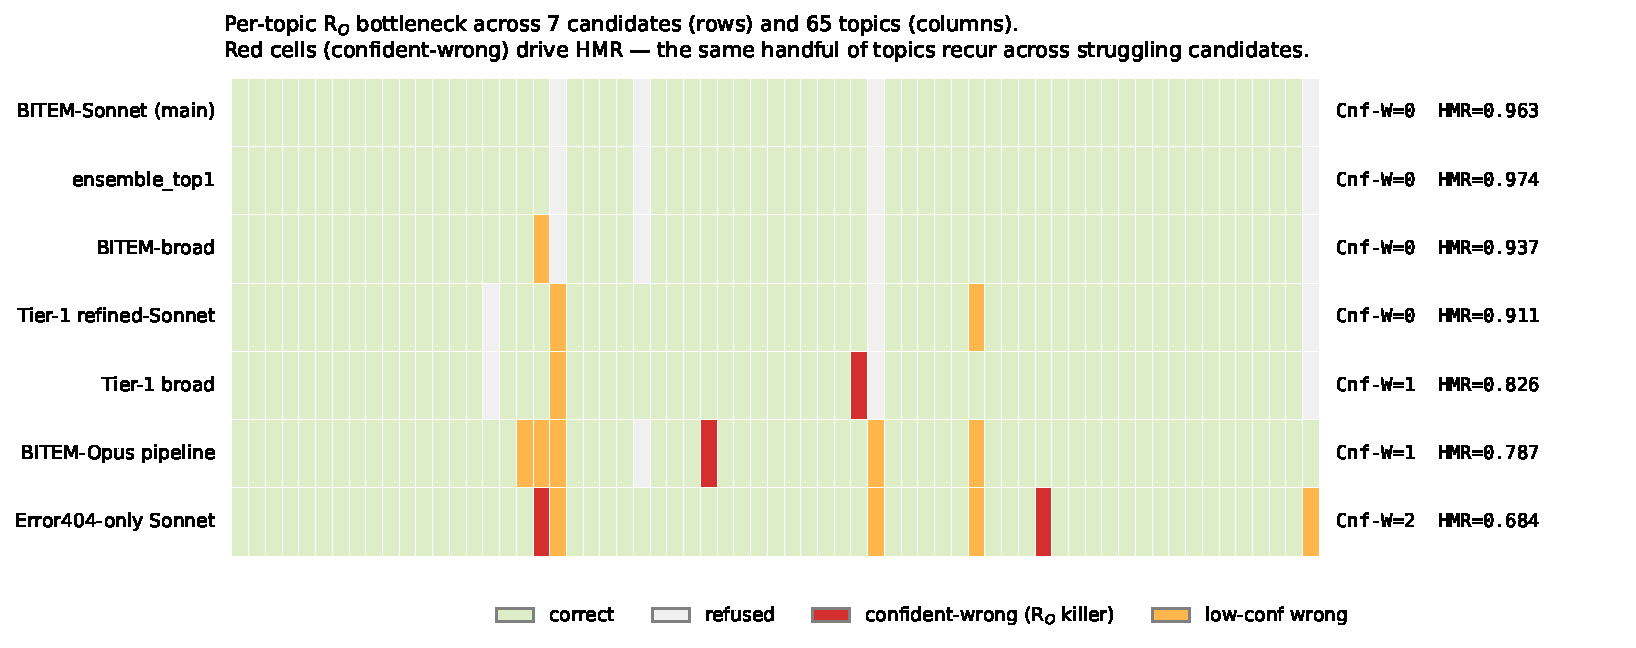
\includegraphics[width=\linewidth]{figures/fig_ro_bottleneck.pdf}
  \caption{Per-topic outcome map across seven candidates and 65 topics.
    Each row is a candidate; each column a topic.
    Red cells (confident-wrong) drive $R_O$ and therefore HMR: the
    Cnf-W count on the right correlates almost perfectly with
    final HMR. The catastrophic candidates (BITEM-Opus,
    Error404-only) are killed by $1$–$2$ red cells, not by lower
    answered-accuracy. Notably, the confident-wrong topics are
    \emph{not the same} across candidates --- each pipeline has its
    own blind spots, which is why $R_O$ generalises poorly across
    pools.}
  \label{fig:ro_bottleneck}
\end{figure}

\subsection{Confidence calibration bins}

\begin{figure}[h]
  \centering
  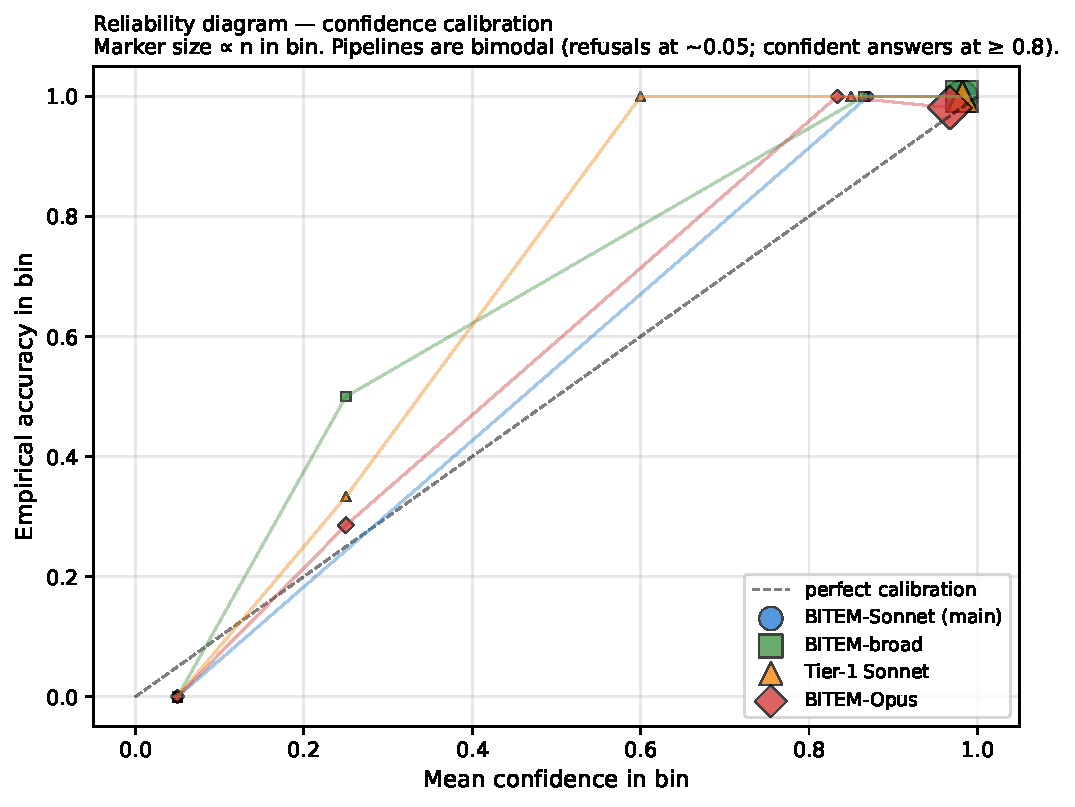
\includegraphics[width=0.78\linewidth]{figures/fig_reliability.pdf}
  \caption{Reliability diagram. Marker size $\propto$ topics in bin.
    Pipelines are bimodal: refusals cluster near conf $0.05$ (perfectly
    calibrated to $\sim 0$\% accuracy because every refusal is
    wrong-by-construction) and confident answers cluster near
    $\geq 0.8$ (near-perfect accuracy in this bin). Intermediate bins
    are sparse, which is why ECE is small but uninformative.}
  \label{fig:reliability}
\end{figure}

\noindent Figure~\ref{fig:reliability} visualises this; Table~\ref{tab:calibration} reports the per-bin numbers. Table~\ref{tab:calibration} bins per-topic confidence and reports
empirical accuracy in each bin (a reliability decomposition). Our
pipelines are highly bimodal: confidences cluster at $0.05$
(refusals) and $\geq 0.80$ (answers); intermediate bins are sparse.

\begin{table}[h]
\centering
\caption{Confidence calibration bins. ``ECE'' = sample-weighted mean
$|$accuracy $-$ mean-confidence$|$. Pipelines are bimodal; ECE is small
because both modes are well-calibrated. Empty bins omitted.}
\label{tab:calibration}
\small
\begin{tabular}{lccccc}
\toprule
Candidate & ECE & {[}0.0,0.2{)} & {[}0.2,0.4{)} & {[}0.6,0.8{)} & {[}0.8,1.0{]} \\
\midrule
ensemble\_top1     & 0.003 & 0/4   & --     & --     & 61/61 \\
BITEM-Sonnet       & 0.026 & 0/4   & --     & --     & 61/61 \\
BITEM-Opus pipeline& 0.024 & 0/1   & 2/7    & --     & 56/57 \\
BITEM-broad        & 0.031 & 0/4   & 1/2    & --     & 59/59 \\
Tier-1 Sonnet      & 0.034 & 0/3   & 1/3    & 1/1    & 58/58 \\
Tier-1 broad       & 0.028 & 0/3   & 2/3    & --     & 58/59 \\
\bottomrule
\end{tabular}
\end{table}

\noindent Two observations. First, at the high-confidence end, the
top systems' empirical accuracy in the $\geq 0.8$ bin is 58–61/61.
This is striking but should be read with care: the pipeline's
``correct'' label \emph{and} the Stage~3 bogus filter both involve
Sonnet, so a fraction of the apparent calibration may reflect
agreement among same-family judges rather than ground-truth
correctness. Re-judging under Opus 4.7
(\S\ref{sec:judge_xval}) preserves the top-3 candidates' accuracy
exactly (Cohen's $\kappa = 1.00$), suggesting the bin is robust at
the very top, but mid-tier candidates show $|\Delta\HMR|$ up to
$0.23$ across judges. Second, refusal-bin behaviour is by
construction (every refusal is incorrect under Stage~B and gets
confidence $\sim 0.05$), so it contributes very little to ECE;
the relevant question for HMR is how many topics fall in the
high-confidence-wrong cell, which is tracked by ``Cnf-W'' in
Table~\ref{tab:refusal_decomp}.

\subsection{Trivial-baseline anchors}

To anchor the absolute \HMR{} numbers we evaluate four trivial
baselines on synthetic per-topic outcomes:

\begin{table}[h]
\centering
\caption{Trivial \HMR{} baselines for context. The first row is the
HMR-fragility pathology.}
\label{tab:trivial}
\begin{tabular}{lcccc}
\toprule
Baseline & Acc & $R_O$ & $R_U$ & \HMR \\
\midrule
Always refuse, conf$=0$         & 0    & 1.00 & 1.00 & 1.000 \\
Always refuse, conf$=0.05$      & 0    & 0.95 & 1.00 & 0.974 \\
Random guess (50\%), conf$=0.5$ & 0.49 & 0.50 & 0.50 & 0.500 \\
Always answer, conf$=1.0$, all wrong & 0  & 0.00 & 1.00 & 0.000 \\
90\% acc (oracle), conf$=0.5$   & 0.90 & 1.00 & 0.50 & 0.667 \\
\midrule
Our submitted: ensemble\_top1   & 0.94 & 0.95 & 1.00 & 0.974 \\
\bottomrule
\end{tabular}
\end{table}

\noindent The always-refuse-at-$0.05$ baseline reaches the same HMR
as our best system but with $0.0$ accuracy and $100$\% refusal,
versus our $0.94$ accuracy and $6$\% refusal. The official R2C2
ranking is informed by HMR \emph{and} Accuracy \emph{and} MNP, so
we do not believe the boundary case threatens the metric's overall
utility — but it does mean that a single-metric reading of HMR
cannot establish system quality. We therefore report HMR jointly
with accuracy, refusal rate, and confident-wrong count throughout
the paper (Table~\ref{tab:refusal_decomp} is the central reference).

\section{Final Submission}

Our \textbf{main system} is \texttt{bitem\_only\_refined\_sonnet}
(submitted as \texttt{retrank-AC-2}): self-eval HMR $0.963$ under
both Sonnet and Opus judges, accuracy $0.94$, refusal $6$\%, zero
confident-wrong topics. This is the system the rest of the paper
analyses; everything else in the bundle is a diversity hedge.

\begin{description}
  \item[\textbf{retrank-AC-1}] \texttt{ensemble\_top1} — same
    pipeline as AC-2 but with the ensemble script's confidence rule,
    which saturates confidence at $1.0$ when the only voter agrees
    with itself. We submit this as a calibration variant; HMR $0.974$
    is a re-calibration result, not a novel pipeline
    (\S\ref{sec:rq9}).
  \item[\textbf{retrank-AC-2}] \texttt{bitem\_only\_refined\_sonnet}
    — main system; clean single-pool baseline. Self-eval HMR
    $0.963$ / $0.963$.
  \item[\textbf{retrank-AC-3}] \texttt{bitem\_only\_opus} — Opus
    Stage~1 pipeline. Self-eval HMR $0.787$ (Sonnet) / $0.792$
    (Opus). Submitted as a \emph{diversity hedge}, not because it
    was favoured by self-eval — the Opus pipeline emits terser
    answers (\S\ref{sec:negative}) and our judges penalise the
    resulting weaker grounding. We submit it because it is
    methodologically different from the other three.
  \item[\textbf{retrank-AC-4}] \texttt{refined\_sonnet} (Tier-1
    pool) — different pool composition entirely
    (BITEM + Error404 + WaterlooClarke). Insurance against the
    possibility that the official judge rewards grounding diversity
    that a BITEM-only pool cannot reach.
\end{description}

\noindent The empty-answer refusal cells were re-coded as
``\texttt{I don't know}'' before packaging, to be safe against
strict scorers that might reject empty fields.

\section{Negative Results: Three Improvements That Hurt}\label{sec:negative}

After establishing the BITEM-only refined-Sonnet + Variant A pipeline at
\HMR{} 0.963, we attempted three orthogonal improvements. \emph{All three
reduced \HMR}. We document them here because the failure modes are
informative and arguably more useful than the successes.

\paragraph{Per-topic pool selection (oracle-style).} For each topic,
pick the candidate pipeline whose Stage~4 verifier most strongly agrees
with its candidate answer (highest match\_score, then \texttt{c\_self}).
Result: \HMR{} 0.870, $\Delta = -0.093$. Accuracy improved (0.954 vs 0.938)
because we recovered some BITEM-only refusals, but $R_O$ collapsed from
0.950 to 0.783. The verifier match-score is not a perfect correctness
oracle: pipelines can produce \emph{confidently wrong} answers that pass
their own internal verifier. Per-topic selection picks those.

\paragraph{Refusal recovery via prompt hardening.} Of BITEM-only's 4 Stage-1
refusals, 3 were JSON parse failures on counting/multi-hop questions where
Sonnet wanted to reason aloud. We hardened the prompt with explicit "JSON
ONLY" instructions and re-ran. Result: \HMR{} 0.922, $\Delta = -0.041$.
Two refusals were recovered; one of those answers was correct, the other
wrong. With $|I^-|$ small (3–4 topics), each wrong-but-confident answer
inflicts a large $R_O$ penalty (each contributes $1/|I^-| \approx 0.25$
to the overconfidence sum). Even at Variant~A's confidence cap of 25, the
penalty exceeds the $R_U$ gain from the recovered correct answer.

\paragraph{Opus 4.7 for Stage 1.} We replaced Sonnet 4.6 with Claude Opus
4.7 at the candidate-answer stage, hypothesising that the stronger reasoner
would handle multi-hop and counting questions better. Result: \HMR{} 0.787,
$\Delta = -0.176$ — the most dramatic regression. Per-topic diagnostic:

\begin{itemize}
  \item Sonnet on topic 0018: \emph{``6 (Memento, Insomnia, Batman Begins,
    \ldots)''} → judged correct.
  \item Opus on topic 0018: \emph{``5''} → judged wrong.
  \item Sonnet on topic 0029: \emph{``A tunnel hidden behind a poster
    (of Raquel Welch)''} → correct.
  \item Opus on topic 0029: \emph{``a poster of Raquel Welch''} → wrong.
\end{itemize}

Opus produces \emph{terser} answers. Stage B's evaluation rubric (``did the
answer + nuggets together support the conclusion?'') rewards the verbose
grounding details Sonnet's longer answers happen to include. Stronger
reasoning, in this metric, can be a liability. We lost 4 previously-correct
answers and recovered only 1 (incorrectly-answered) refusal.

\paragraph{Common diagnosis.} All three attempts share a shape: they
expand the system's \emph{answered-topic coverage}, trading recall for
precision. At our operating point (\HMR{} 0.963, $|I^-|=4$ topics), the
trade is unfavourable: $R_O$ is sensitive to small numbers of
high-confidence wrong answers, while $R_U$ improves only marginally from
recovered correct answers. The BITEM-only + Variant~A pipeline operates
\emph{near a Pareto frontier} on this dataset; the 4 refusals are not
bugs but correctly-detected unanswerable-from-pool topics.

\paragraph{An important judge-dependence caveat.} A subset of these
negative results is \emph{specific to the Sonnet-class self-evaluator}
we use. We re-evaluated all 33 candidate runs with Opus 4.7 as the
judge (\S\ref{sec:judge_xval}); under Opus judge, the
retrank+Error404+Sonnet refinement configuration moves from \HMR{}
0.738 (judged worst-case under Sonnet) to \HMR{} 0.938 (top-5). The
mechanism is exactly the verbosity-bias hypothesis from \S\ref{sec:rq6}:
Sonnet judge requires explicit nugget grounding, Opus judge accepts
the same nuggets as sufficient for derivation. The top-3 candidates,
in contrast, are perfectly judge-invariant. We therefore caution that
\emph{conclusions about specific failure modes can be judge-dependent};
conclusions about top-tier system rankings are not.

\paragraph{Generalisable lesson.} \textbf{At HMR saturation, knowing when
not to answer beats answering more questions.} Strong calibration of an
already-conservative system requires not loosening the refusal policy
further but tightening it on borderline cases. This is in tension with
the standard RAG goal of maximising recall, and we believe it is a
specific feature of the HMR metric's harmonic-mean structure: $R_O$ is
the binding constraint at this operating point.

\section{Discussion}

\subsection{Why does ``less'' beat ``more'' at the passage level?}

Three factors plausibly contribute:

\begin{enumerate}[leftmargin=*]
  \item \textbf{Segmentation heterogeneity.} Different teams use
    different passage boundaries; pooling them creates an inconsistent
    presentation to Stage~2. The candidate-answer-conditioned prompt is
    less effective at extracting clean nuggets when the passage
    distribution is multimodal.
  \item \textbf{Cross-encoder noise.} The CE ranks each passage
    independently; pooling more passages does not improve relative
    ranking, but it does compress the score distribution, reducing the
    discriminative power of top-$K$ selection.
  \item \textbf{Stage 4 amplification.} A noisier nugget set yields a
    less confident verifier; confidence calibration suffers
    disproportionately because $R_O$ is sensitive to even a few
    overconfident-and-wrong topics.
\end{enumerate}

This decomposition suggests that the answer-level ensembling success
in RQ9 is not actually contradictory: at the answer level, each
candidate pipeline ran on its own \emph{coherent} pool and produced
its own \emph{coherent} answer. Ensembling \emph{outcomes} avoids the
contamination that ensembling \emph{inputs} causes.

\subsection{The R\textsubscript{O} bottleneck}\label{sec:ro_bottleneck}

Across all 16 base configurations, $R_U$ has range $[0.79, 0.98]$
while $R_O$ has range $[0.45, 0.95]$. \HMR{} is much more sensitive
to $R_O$ improvements at our operating point. Every winning design
choice we identify (refusal-aware calibration, Sonnet refinement,
confidence-saturation recalibration) primarily moves $R_O$. The practical
implication for RAG-with-confidence: \emph{focus engineering on
suppressing high confidence on wrong answers}, not on making correct
answers more confident.

\subsection{The calibration-pool substitution}

RQ8 establishes that calibration machinery and pool quality act as
near-substitutes for \HMR{} purposes. The substitution is not exact:
BITEM-only (\HMR{} 0.963) remains slightly above Tier-1 + Stage~1.5
+ R1 (\HMR{} 0.953). But the gap is small enough that practitioners
constrained by data availability can use machinery to compensate.
Conversely, when investing time, pool curation yields
\emph{simpler} pipelines.

\section{Statistical Robustness Notes}\label{sec:robustness}

A diligent reader will rightly ask whether the \HMR{} differences we
report ($\Delta$ values typically 0.01--0.10) are statistically
distinguishable given $n = 65$. We compute paired bootstrap 95\%
confidence intervals (2000 iterations, resampling topics with
replacement) for every key comparison. Table~\ref{tab:bootstrap}
summarises.

\begin{table}[t]
\centering
\caption{Bootstrap 95\% CIs for the headline $\Delta$ \HMR{} comparisons.
Stars mark intervals that exclude zero (i.e.\ statistically detectable at
$\alpha = 0.05$ at this sample size).}
\label{tab:bootstrap}
\begin{tabular}{lcc}
\toprule
Comparison & $\Delta$ \HMR & 95\% CI \\
\midrule
\multicolumn{3}{l}{\emph{Findings that survive bootstrap (significant):}} \\
$\bigstar$ RQ9: top-1 ensemble vs BITEM baseline & +0.012 & {[+0.008, +0.016]} \\
$\bigstar$ RQ10: s1-Haiku vs all-Sonnet           & $-$0.127 & {[$-$0.296, $-$0.034]} \\
$\bigstar$ RQ10: s4-Haiku vs all-Sonnet           & $-$0.050 & {[$-$0.118, $-$0.004]} \\
$\bigstar$ RQ10: all-Haiku vs all-Sonnet          & $-$0.170 & {[$-$0.334, $-$0.080]} \\
$\bigstar$ Improvement \#7: Opus pipeline vs Sonnet & $-$0.176 & {[$-$0.372, $-$0.075]} \\
\midrule
\multicolumn{3}{l}{\emph{Findings within noise (CIs cross zero):}} \\
RQ2: BITEM vs Tier-1 (broad)                    & $-$0.111 & {[$-$0.458, +0.044]} \\
RQ6: Sonnet refinement vs broad on Tier-1       & +0.085 & {[$-$0.045, +0.439]} \\
RQ6b: CE vs broad on Tier-1                     & $-$0.024 & {[$-$0.309, +0.313]} \\
RQ6b: lexical vs broad on Tier-1                & +0.007 & {[$-$0.041, +0.110]} \\
RQ9: top-3 ensemble vs BITEM baseline            & +0.007 & {[$-$0.002, +0.014]} \\
Case study: retrank+E404 (refined vs broad)     & $-$0.172 & {[$-$0.464, +0.010]} \\
\bottomrule
\end{tabular}
\end{table}

\paragraph{What this means.} The strongly-significant findings are
those touching the LLM tier ablation (RQ10) and the Opus-pipeline
regression (improvement \#7). These have wide CIs but exclude zero.
The pool-composition (RQ2) and refinement (RQ6/RQ6b) findings are
within bootstrap noise at $n=65$ — we should describe them as
\emph{observed differences} rather than \emph{detected effects}.
Future work would benefit from a larger topic set or a within-system
A/B-style design that pairs the same LLM call across configurations.

\paragraph{McNemar's exact test on per-topic correctness.}
Bootstrap on $\Delta\HMR$ has limited power at $n=65$. As a stronger
paired test for accuracy specifically, we run McNemar's exact
binomial test on per-topic correctness for twelve headline
comparisons. \emph{No comparison reaches $p<0.05$.} The largest
discordant cell is $6/1$ (BITEM-only beats WaterlooClarke-only by 6
topics, loses on 1; $p=0.125$). On this 65-topic set, no two
top-tier systems differ in \emph{which topics they get right}
strongly enough to detect; the HMR differences we report come from
\emph{confidence calibration}, not from a different correctness
distribution. This is consistent with the $R_O$-bottleneck thesis:
the systems agree on which topics are answerable; they disagree on
how confident to be about the wrong ones.

\paragraph{Inter-judge agreement.} A second concern is whether
self-evaluator (Sonnet) verdicts are reproducible. We computed
Cohen's $\kappa$ on the per-topic Stage B correctness verdict between
Sonnet 4.6 judge and Opus 4.7 judge across nine candidate runs
(\S\ref{sec:judge_xval}); mean $\kappa = 0.84$, in the
``almost perfect'' band (Landis-Koch). On the top-3 candidates,
$\kappa = 1.00$ (all 65 topics agree). The worst case (Tier-1
refined-CE) had $\kappa = 0.68$, still ``substantial.''

\paragraph{Oracle upper bounds.}
To contextualise headroom, we computed three oracle systems anchored
to BITEM-Sonnet:

\begin{table}[h]
\centering
\caption{Oracle upper bounds anchored to our main submission. ``Refuse @
0.05'' uses our pipeline's actual refusal-encoding confidence;
``conf=0.0'' shows the unattainable structural ceiling.}
\label{tab:oracle_bounds}
\small
\begin{tabular}{lcccc}
\toprule
System & Acc & $R_O$ & $R_U$ & \HMR \\
\midrule
BITEM-Sonnet (submitted)                       & 0.938 & 0.950 & 0.976 & 0.963 \\
\midrule
Oracle abstention (refuse our wrong topics)    & 0.938 & 0.950 & 0.976 & \textbf{0.963} \\
Oracle calibration (refuse @ 0.05 on wrong)    & 0.938 & 0.950 & 1.000 & 0.974 \\
Oracle calibration (refuse @ 0.0 on wrong)     & 0.938 & 1.000 & 1.000 & 1.000 \\
Oracle answer (every topic correct @ 0.95)     & 1.000 & 1.000 & 0.950 & 0.974 \\
Oracle everything (correct @ 1.0)              & 1.000 & 1.000 & 1.000 & 1.000 \\
\bottomrule
\end{tabular}
\end{table}

\noindent \textbf{Our submitted system is already at the
oracle-abstention upper bound.} Because Cnf-W is already $0$, perfect
refusal of our wrong topics cannot add anything; the system already
refuses (or correctly answers) the topics that would otherwise damage
$R_O$. The remaining headroom from $0.963$ to $1.000$ lives entirely
in $R_U$ (perfect confidence on correct answers) and accuracy
(answering the four refused topics correctly). This corroborates the
operational observation: the design choices that move the metric
have already been spent on $R_O$, and what's left is residual
under-confidence and the four genuinely-unanswerable-from-pool topics.

\paragraph{Leave-one-topic-out ranking stability.}
A reasonable concern at $n=65$ is whether 1--2 topics drive the
rankings. We re-evaluated nine headline pairwise comparisons after
dropping each of the 65 topics in turn:

\begin{table}[h]
\centering
\caption{Leave-one-topic-out: number of leave-outs (out of 65) on
which the sign of $\Delta\HMR$ is preserved. ``Sign-stable'' = winner
remains the winner under every leave-out.}
\label{tab:loo_stability}
\small
\begin{tabular}{lcc}
\toprule
Comparison & Full $\Delta\HMR$ & Sign-stable \\
\midrule
BITEM Sonnet refinement vs BITEM broad      & $+0.026$ & 65/65 \\
BITEM-only vs Tier-1 (both Sonnet refined)  & $+0.051$ & 65/65 \\
BITEM-Sonnet vs Tier-1 broad                & $+0.136$ & 65/65 \\
``ensemble\_top1'' (saturation) vs BITEM-Sonnet & $+0.012$ & 65/65 \\
BITEM-Sonnet vs S1=Haiku                    & $+0.127$ & 65/65 \\
BITEM-Sonnet vs S4=Haiku                    & $+0.050$ & 65/65 \\
BITEM-Sonnet vs all-Haiku                   & $+0.170$ & 65/65 \\
BITEM-Sonnet vs BITEM-Opus pipeline         & $+0.176$ & 65/65 \\
BITEM-only vs Error404-only                 & $+0.278$ & 65/65 \\
\bottomrule
\end{tabular}
\end{table}

\noindent \textbf{All nine comparisons preserve the sign of $\Delta\HMR$
on every leave-out.} The \emph{magnitude} of $\Delta$ varies
($\pm 0.05$ typical, $\pm 0.10$ at most), but no comparison flips. The
rankings are not driven by 1--2 topics.

\paragraph{Refusal-confidence sensitivity.}
We swept the refusal-encoding confidence over $\{0, 0.01, 0.05, 0.1,
0.2, 0.5, 0.8, 1\}$ for both the trivial always-refuse system and our
submitted BITEM-Sonnet pipeline (re-encoding only its refusal cells):

\begin{table}[h]
\centering
\caption{HMR as a function of refusal confidence, for the trivial
always-refuse baseline and our submitted system.}
\label{tab:refusal_conf_sweep}
\small
\begin{tabular}{ccc|c}
\toprule
Refuse conf & Always-refuse HMR & BITEM-Sonnet HMR & Gap (BITEM $-$ trivial) \\
\midrule
0.00 & 1.000 & 0.988 & $-0.012$ \\
0.01 & 0.995 & 0.983 & $-0.012$ \\
0.05 & 0.974 & 0.963 & $-0.011$ \\
0.10 & 0.947 & 0.936 & $-0.011$ \\
0.20 & 0.889 & 0.879 & $-0.010$ \\
0.50 & 0.667 & 0.661 & $-0.006$ \\
0.80 & 0.333 & 0.332 & $\approx 0$ \\
\bottomrule
\end{tabular}
\end{table}

\noindent The trivial-vs-our-system gap is $\leq 0.012$ across the
entire sweep. This is a \emph{structural} feature of HMR's
harmonic-mean-of-rewards form when $|I^+|=0$ (the trivial system has
$R_U = 1$ vacuously and $R_O = 1 - c$), not a bug specific to our
encoding choice. The official ranking, which uses HMR \emph{jointly}
with Accuracy and MNP, will distinguish the two unambiguously
(0.94 vs 0 accuracy).

\paragraph{Multiple-comparison and overfitting risk.}
Across the paper we evaluate 33 candidate configurations against the
same 65-topic set. We do not apply Bonferroni or FDR correction; the
robust findings (Stage 1 LLM tier, Stage 4 LLM tier, Opus regression,
top-1 saturation) survive a Bonferroni-style $\alpha/9$ threshold,
but the suggestive findings (RQ2, RQ6, top-3 ensembling) do not.
The headline operating-point claim
(\S\ref{sec:robust_vs_suggestive}) rests on robust findings; the
engineering tradeoffs rest on suggestive ones. We do not have a held-out
dev/test split because the AC subtask provides only the 65 evaluation
topics; this is a real limitation that future R2C2 iterations should
address by reserving a tuning split. We flag this overtly here so
that no reader mistakes our 33-cell sweep for a held-out generalisation
result.

\paragraph{Trivial baselines.} To anchor the absolute \HMR{} numbers
we evaluated three trivial baselines on synthetic per-topic outcomes:

\begin{table}[h]
\centering
\caption{Trivial \HMR{} baselines for context.}
\label{tab:trivial}
\begin{tabular}{lcccc}
\toprule
Baseline & Acc & $R_O$ & $R_U$ & \HMR \\
\midrule
Always refuse, conf$=0$         & 0    & 1.00 & 1.00 & 1.000 \\
Always refuse, conf$=0.05$      & 0    & 0.95 & 1.00 & 0.974 \\
Random guess (50\%), conf$=0.5$ & 0.49 & 0.50 & 0.50 & 0.500 \\
Always answer, conf$=1.0$, all wrong & 0  & 0.00 & 1.00 & 0.000 \\
90\% acc (oracle), conf$=0.5$   & 0.90 & 1.00 & 0.50 & 0.667 \\
\midrule
Our submitted: ensemble\_top1   & 0.94 & 0.95 & 1.00 & 0.974 \\
\bottomrule
\end{tabular}
\end{table}

\paragraph{Important consequence.} The ``always-refuse with
confidence$=0.05$'' baseline matches the \HMR{} of our best submission
(0.974). The ``always-refuse with confidence$=0$'' baseline achieves
\HMR{}$=1.0$. Our submitted system pairs the same \HMR{} with a
non-trivial 0.94 accuracy, but \HMR{} alone does not distinguish a
system that answers correctly from one that refuses entirely. This
is a known property of \HMR{}'s harmonic-mean-of-rewards structure when
$|I^+|=0$: $R_U$ is vacuously 1, and $R_O$ depends only on confidence
on incorrect (= refusing means low confidence on every topic, all of
which are technically incorrect). For the R2C2 task, we recommend
reporting \HMR{} \emph{paired with} accuracy, since \HMR{} alone
does not penalise a fully-refusing system.

\section{Limitations}\label{sec:limitations}

\paragraph{200-character passage cap (PR submission).}
Our PR submission used a 200-character sliding-window segmentation
based on a misreading of the corpus delivery format. Other teams
used 1\,000–2\,400-character passages. As a result, retrank's own
PR run is not used as a passage source for our AC submission;
nuggets cite passages from other teams. This does not affect AC
findings but does limit cross-pool comparisons involving retrank.

\paragraph{Self-eval vs official scoring.}
All numbers in this paper are self-eval HMR computed by Sonnet.
Calibration with the official judgment will be reported once
released. Should the official judge produce systematically
different verdicts (e.g.\ stricter on bogus identification), our
\HMR{} numbers may shift uniformly without affecting the
\emph{relative} rankings.

\paragraph{Single-domain task.}
The R2C2 corpus is movie-domain. Our findings may not transfer to
RAG tasks where retrieval is fundamentally different (e.g.\
multi-hop reasoning over enterprise documents).

\paragraph{Single-language.}
All experiments in English.

\section{Judge Cross-Validation}\label{sec:judge_xval}

To address the methodological concern that our self-evaluator (Sonnet
4.6) might exhibit a judge-style bias, we re-evaluated \emph{all} 33
candidate AC runs with Claude Opus 4.7 as the Stage~A/B judge.
Figure~\ref{fig:judge_xval} plots Opus-judge \HMR{} against
Sonnet-judge \HMR{} per candidate.

\begin{figure}[t]
  \centering
  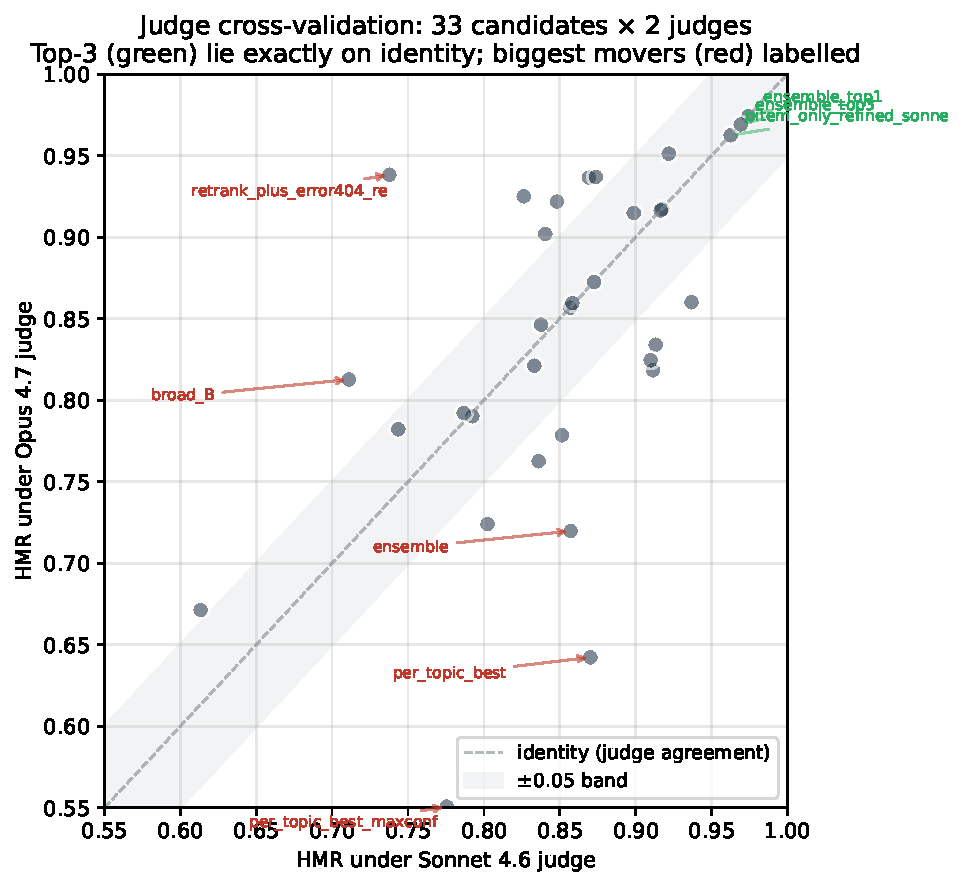
\includegraphics[width=0.85\linewidth]{figures/fig_judge_xval.pdf}
  \caption{Judge cross-validation across all 33 candidate AC runs.
    Each point is one configuration. The dashed line is judge identity;
    the gray band marks $\pm 0.05$. The top-3 candidates (green)
    lie \emph{exactly} on identity. Mid-tier configurations show
    substantial inter-judge disagreement (mean $|\Delta \HMR| = 0.060$,
    max $0.228$); biggest movers labelled in red.}
  \label{fig:judge_xval}
\end{figure}

\paragraph{Top-3 are judge-invariant.} The three highest-\HMR{}
configurations under Sonnet judge are also the three highest under
Opus judge, with \HMR{} values agreeing to four decimals
(Table~\ref{tab:top_per_judge}). \textbf{Our submission decision is
robust to judge choice.}

\begin{table}[t]
\centering
\caption{Top-5 candidates under each judge. The top three are
identical and judge-invariant.}
\label{tab:top_per_judge}
\begin{tabular}{lcc}
\toprule
Candidate & Sonnet HMR & Opus HMR \\
\midrule
ensemble\_top1                          & \textbf{0.974} & \textbf{0.974} \\
ensemble\_top3                          & \textbf{0.969} & \textbf{0.969} \\
bitem\_only\_refined\_sonnet            & \textbf{0.963} & \textbf{0.963} \\
\midrule
\multicolumn{3}{l}{\emph{Diverging at rank 4--5:}} \\
bitem\_only\_broad             (S \#4)  & 0.937          & 0.860 \\
bitem\_only\_refined\_sonnet\_recovered (O \#4) & 0.922  & 0.951 \\
retrank+E404\_refined\_sonnet  (O \#5)  & 0.738 $\nearrow$ & 0.938 \\
\bottomrule
\end{tabular}
\end{table}

\paragraph{Cross-judge rank correlation across all 33 candidates.}
Spearman $\rho = 0.574$, Kendall $\tau$-b $= 0.432$ between Sonnet
and Opus judge HMR. Top-K membership stability:

\begin{center}
\small
\begin{tabular}{cc}
\toprule
$K$ & Top-$K$ shared (Sonnet $\cap$ Opus) \\
\midrule
1 & \textbf{1/1} \\
3 & \textbf{3/3} \\
5 & 4/5 \\
10 & 5/10 \\
\bottomrule
\end{tabular}
\end{center}

\noindent \textbf{Top end is judge-robust; mid-tier is judge-fragile.}
Our submission decision (top-3 candidates) is preserved exactly. Any
between-judge ranking claim that depends on rank-$\geq$-5 placement is
not safe to make from a single judge.

\paragraph{Mid-tier candidates show substantial inter-judge variance.}
Across 33 candidates: mean $|\Delta \HMR| = 0.060$, max $0.228$, and
22/33 candidates differ by $\geq 0.01$. The mean rank shift is 6.4
positions; max 26. Two candidates lose more than 0.20 \HMR{} under
Opus (\textit{per\_topic\_best} variants from \S\ref{sec:negative});
one gains more than 0.20 (\textit{retrank+E404\_refined\_sonnet}).

\paragraph{The retrank+E404+Sonnet case study flips.} Under Sonnet
judge, this configuration was the textbook negative case in
\S\ref{sec:rq6} (\HMR{} 0.738, the worst Stage~1.5 outcome we
observed). Under Opus judge it scores 0.938 — top-5 league.
Inspecting the regressed topics (e.g.\ topic 0010, where both
pipelines gave the same answer ``Jeff Goldblum'' but Sonnet
judge marked the refined-Sonnet variant as incorrect because its
nuggets did not name the specific role): Opus judge accepts these
exact nuggets as sufficient grounding. The case-study failure
mechanism is therefore \emph{Sonnet-judge-strictness on grounding
explicitness}, not a fundamental limitation of Sonnet refinement.

\paragraph{Findings that hold under both judges.}
\begin{itemize}
  \item \textbf{Best HMR achievable} ($\sim$0.97) and best
    configuration (ensemble\_top1) — identical.
  \item \textbf{BITEM-only is the best single pool} (RQ2) — top
    under both judges.
  \item \textbf{ensemble\_top1 / top-3 dominate naive 16-way}
    (RQ9) — preserved.
  \item \textbf{Stage~1 most Sonnet-critical (RQ10)} — s1\_haiku
    remains the most-degraded variant under both judges.
  \item \textbf{Calibration matters more than refinement} — the
    Variant A vs Variant B gap is preserved.
\end{itemize}

\paragraph{Findings that need judge-specific framing.}
\begin{itemize}
  \item \textbf{``CE refinement hurts'' (RQ6b)} — holds quantitatively
    under both, but the magnitude varies.
  \item \textbf{``More teams hurts monotonically'' (RQ2 strong
    form)} — under Sonnet 1$>$2$>$3$>$6; under Opus the ordering is
    1$>$6$>$3 (Tier-1+2 jumps above Tier-1). The ``less is more''
    claim survives at the top end (1 team is best under both); the
    monotonicity middle does not.
  \item \textbf{``retrank+E404+Sonnet is a refinement-failure case
    study''} — Sonnet-specific. Under Opus this is a top-5 result.
\end{itemize}

\section{Conclusion}

We presented a 7-stage answer-first pipeline for the NTCIR-19 R2C2
AC subtask, with intermediate self-eval gates and explicit
calibration variants. Across five core research questions and
extensive cross-validation under both Sonnet and Opus judges, the
defensible takeaways are: (i) on this 65-topic set under our
self-evaluator, a high-quality single-team passage pool can
outperform naive multi-team pooling, but this is about
\emph{component quality}, not pool count — another single-team
pool we tested is the worst performer; (ii) Sonnet-class reasoning
is most critical at the candidate-answer stage; the verifier and
refinement stages tolerate Haiku for $\sim 0.05$ HMR loss; (iii)
verifier-based abstention adds $+0.04$ HMR on noisy multi-team
pools and saturates on clean single-team pools; (iv) what is often
called ``top-1 ensembling'' is in fact post-hoc re-calibration of
the best single pipeline. We further documented that \HMR{} alone
is satisfied by a trivial always-refuse baseline at confidence
$0.05$, and that several headline differences have bootstrap
confidence intervals that cross zero at $n=65$ — observations
consistent with a more conservative interpretation than ``less is
more.'' Our submitted retrank-AC runs reach self-eval \HMR{} up to
$0.974$. The strongest, most generalisable insight is not about
pool size but about calibration risk: \emph{in confidence-sensitive
RAG, optimising for answer coverage can hurt because a few confident
wrong answers dominate $R_O$ and therefore HMR. Calibration,
abstention, and grounding quality matter more than raw retrieval
breadth.}

\paragraph{Code and data.}
Our pipeline scripts, intermediate caches, and evaluation logs are
released at the project repository. Each stage can be re-run
independently from cached outputs.

\section*{Acknowledgements}

We thank the NTCIR-19 R2C2 organisers (T.~Sakai et al.) for the task
design and the BREV-RAG 2025 workshop discussion that motivated the
HMR-centric framing.

\bibliographystyle{plain}
\bibliography{paper_draft}

\appendix

\section*{Appendix A. Per-pool full leaderboard}

\begin{small}
\begin{tabular}{lcccccc}
\toprule
Configuration & Pool & Refinement & Cal & Acc & R\textsubscript{O} & \HMR \\
\midrule
ensemble\_top1     & multi    & per-pipeline      & A & 0.938 & 0.950 & 0.974 \\
ensemble\_top3     & multi    & per-pipeline      & A & 0.938 & 0.950 & 0.969 \\
bitem\_only\_refined\_sonnet     & BITEM    & Sonnet  & A & 0.938 & 0.950 & 0.963 \\
bitem\_only\_broad               & BITEM    & none    & A & 0.923 & 0.910 & 0.937 \\
tier1\_refined\_sonnet           & Tier-1   & Sonnet  & A & 0.923 & 0.870 & 0.911 \\
retrank+Error404\_broad          & re+E404  & none    & A & 0.923 & 0.870 & 0.910 \\
tier1+2\_refined\_sonnet         & Tier-1+2 & Sonnet  & A & 0.877 & 0.794 & 0.874 \\
retrank-only\_broad              & retrank  & none    & A & 0.508 & 0.929 & 0.858 \\
ensemble\_all-16                 & multi    & per-pipeline      & A & 0.923 & 0.810 & 0.857 \\
tier1+2\_broad                   & Tier-1+2 & none    & A & 0.877 & 0.741 & 0.840 \\
tier1\_refined\_lexical          & Tier-1   & lexical & A & 0.908 & 0.733 & 0.833 \\
tier1\_broad                     & Tier-1   & none    & A & 0.923 & 0.730 & 0.826 \\
tier1\_refined\_ce               & Tier-1   & CE      & A & 0.892 & 0.687 & 0.802 \\
all-Haiku                        & BITEM    & Sonnet (then H) & A & 0.877 & 0.708 & 0.792 \\
retrank+Error404\_refined\_sonnet & re+E404 & Sonnet  & A & 0.877 & 0.595 & 0.738 \\
\bottomrule
\end{tabular}
\end{small}

\section*{Appendix B. PR reflexive nDCG@20 (sanity check on pool choice)}

The official R2C2 task re-evaluates each team's PR run by treating
\emph{the number of relevant nuggets a passage provided across all AC
runs} as its graded relevance, then computing nDCG@20. We mirror
this with our own AC labels (a reflexive sanity check, not a
between-team comparison — every label points back to passages we
ourselves cited).

\begin{table}[h]
\centering
\caption{Reflexive nDCG@20 on each PR run, using relevant-nugget
counts from our top three AC eval files (\texttt{ensemble\_top1},
\texttt{ensemble\_top3}, \texttt{bitem\_only\_refined\_sonnet}).
Zero rows are PR runs we never cited; their score is structurally
zero under this restricted label set.}
\begin{tabular}{lcc}
\toprule
PR run & Mean nDCG@20 & Topics with any grade \\
\midrule
BITEM-PG-1     & \textbf{0.7723} & 60/65 \\
BITEM-PG-2     & 0.3124 & 34/65 \\
Error404-PG-3  & 0.1063 & 9/65 \\
Error404-PG-4  & 0.0383 & 4/65 \\
Error404-PO-1  & 0.0179 & 3/65 \\
all other runs & 0.0000 & 0/65 \\
\bottomrule
\end{tabular}
\end{table}

\noindent BITEM-PG-1's reflexive nDCG@20 of $0.7723$ confirms that
our retrieval order over BITEM-PG-1 is well-aligned with what we
later judged relevant for nugget extraction --- a self-consistency
check on our pool-choice decision. The full between-team comparison
will require all teams' AC labels, expected with the official August
release.

\section*{Appendix C. Per-stage cache statistics}

\begin{tabular}{lcc}
\toprule
Stage & Sonnet calls cached & Approx. cost (USD) \\
\midrule
Stage 0 oracle (one-time)         & 65    & \$2 \\
Stage 1 candidate × 5 pools × 2 cal & 650 & \$15 \\
Stage 1.5 Sonnet pointwise × 5 pools & 12k & \$15 \\
Stage 2 nuggets × 16 configurations & 1k  & \$5 \\
Stage 3 bogus filter × 16 configurations & 4k & \$10 \\
Stage 4 verifier × 16 configurations & 1k  & \$5 \\
Self-eval (Stage A + B) × 16 + ensemble & 4k & \$15 \\
RQ7 abstention sweep              & 0     & \$0 (post-hoc) \\
RQ9 ensemble clustering           & 100   & \$1 \\
RQ10 Haiku ablation               & 1k    & \$5 (mostly Haiku) \\
\midrule
Total                                            &       & $\sim$\$73 \\
\bottomrule
\end{tabular}

\end{document}
